\documentclass[11pt]{article}

\usepackage[margin=1in]{geometry}
\usepackage{amsmath, amssymb}
\usepackage{booktabs}
\usepackage{longtable}
\usepackage{array}
\usepackage{tabularx}
\usepackage{pdflscape}
\usepackage{xcolor}
\usepackage{hyperref}
\usepackage{enumitem}
\usepackage{caption}
\usepackage{graphicx}
\usepackage{algorithm}
\usepackage{algpseudocode}
\usepackage{placeins}

\hypersetup{
    colorlinks=true,
    linkcolor=blue!60!black,
    citecolor=blue!60!black,
    urlcolor=blue!60!black
}

\setlist[itemize]{leftmargin=1.5em}
\setlist[enumerate]{leftmargin=1.5em}
\renewcommand{\arraystretch}{1.15}

\title{\textbf{A Scalable Python Pipeline for IMU-Based Behavioral Clustering}}
\author{Chuqi Wang}
\date{June 17, 2026 \\ \normalsize revised August 24, 2026}

\begin{document}
\maketitle

\begin{abstract}
This report describes a Python reimplementation of the MATLAB behavioral clustering pipeline. The core representation is preserved: 300\,ms IMU windows are encoded as channel-wise histograms, converted to CDFs, and compared via CDF-L1 distance (equivalent to 1D Wasserstein/EMD). The main addition is a set of scalable Affinity Propagation variants---random-sampled, coreset, k-means, stratified, sparse, and two-level---that avoid the $O(N^2)$ memory cost of full AP while staying close to its output. All methods are evaluated on eight datasets using silhouette score and ARI against full AP; full AP is now computed on seven of the eight datasets (raised from three), from a single dependency-version-pinned run. Beyond cluster-level agreement, random-sampled AP is validated against full AP on population-level behavioral summaries---occupancy and transition-matrix correlation---with an honest look at where it does \emph{not} agree: frame-level and single-exemplar identity. Random-sampled AP is currently the best practical default; k-means and stratified sampling are promising alternatives for datasets where rare behaviors matter.
\end{abstract}

\section{Project Goal}

This project analyzes mouse behavior from wearable inertial measurement unit (IMU) recordings. The central computational task is to partition continuous motion sensor data into short behavioral windows and assign each window to an unsupervised behavioral cluster. These clusters can then be used for downstream analyses, such as comparing behavioral motif usage across control and Parkinsonian mice or across different arena conditions.

The original MATLAB pipeline performs Affinity Propagation clustering using an EMD-based similarity matrix. However, the MATLAB implementation becomes expensive because it computes many pairwise EMD distances and stores an $N \times N$ similarity matrix, where $N$ is the number of behavioral windows. The Python pipeline keeps the same conceptual distance metric while introducing vectorized preprocessing, CDF-based EMD computation, approximate/exact nearest-neighbor search with FAISS, and several scalable AP variants.

\begin{figure}[h]
\centering
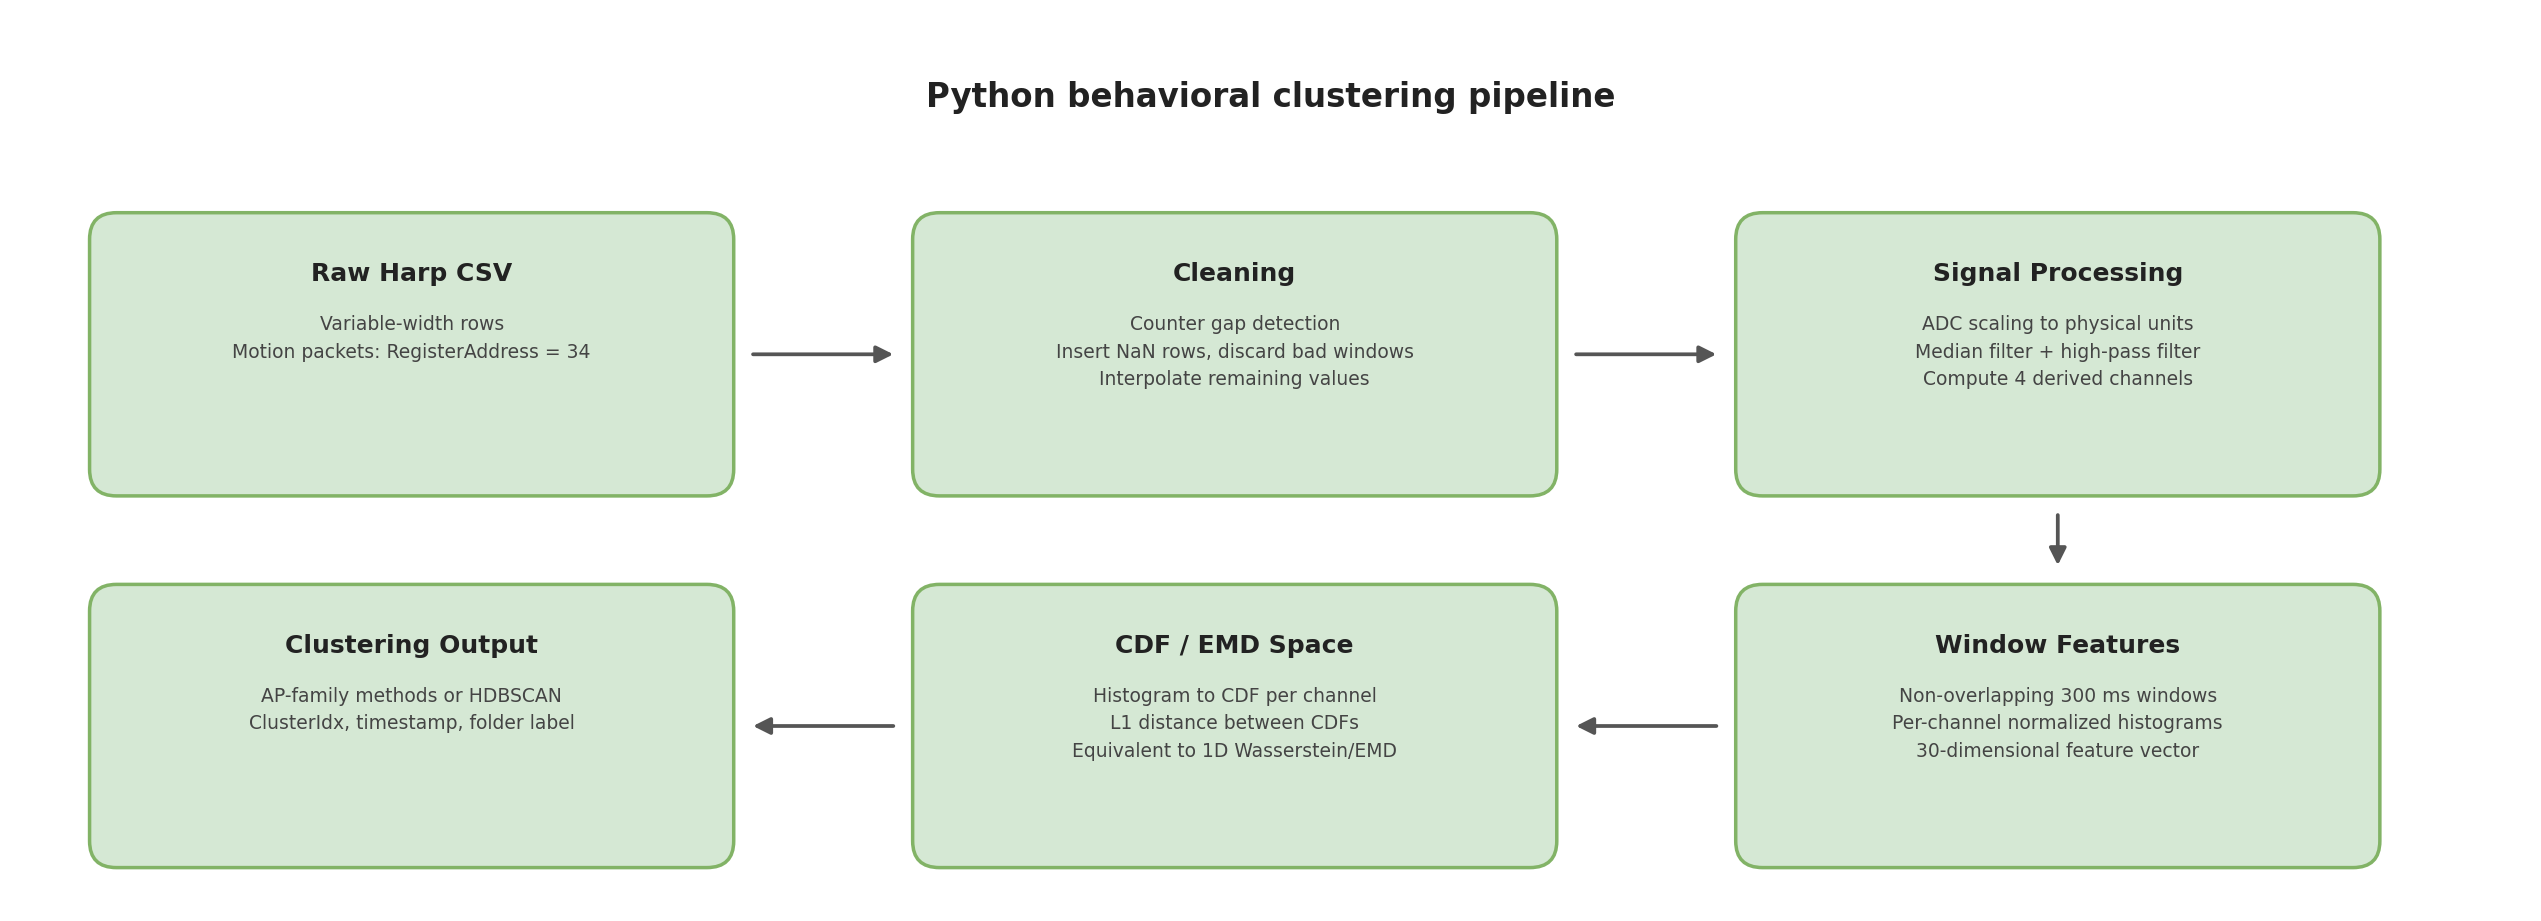
\includegraphics[width=\textwidth]{figures/pipeline_overview.png}
\caption{Overview of the Python pipeline from raw Harp CSV files to behavioral cluster labels.}
\label{fig:pipeline-overview}
\end{figure}

\FloatBarrier
\section{Data Overview}

\subsection{Raw Harp Motion Data}

The raw input is a Harp motion CSV file. Rows can have variable width, so \texttt{prepare\_test\_data.py} first pads all rows into a consistent table. Motion packets are identified by:

\begin{equation}
    \texttt{RegisterAddress} = 34.
\end{equation}

Only these rows contain IMU motion samples. After filtering to motion rows, the Python loader extracts:

\begin{equation}
    \texttt{raw\_motion} \in \mathbb{R}^{N_{\mathrm{samples}} \times 10},
\end{equation}

with columns

\begin{center}
\texttt{[ax, ay, az, gx, gy, gz, mx, my, mz, counter]}.
\end{center}

The first three columns are accelerometer readings, the next three are gyroscope readings, the next three are magnetometer readings, and the last column is the packet counter. Timestamps and folder/session labels are stored separately. The magnetometer columns (\texttt{mx}, \texttt{my}, \texttt{mz}) are present in the raw data but are not used by the current pipeline.

\subsection{Missing-Packet Detection and Cleaning}

The packet counter wraps around from 127 to 0. Consecutive motion packets should therefore have counter difference:

\begin{equation}
    \Delta c = (c_{t+1} - c_t) \bmod 128 = 1.
\end{equation}

If $\Delta c > 1$, then $\Delta c - 1$ motion packets were dropped. The preprocessing script inserts placeholder rows with NaN sensor values and linearly interpolated timestamps. This preserves temporal alignment before windowing.

The cleaning rule is window-based. Since one behavioral window contains 60 samples, corresponding to 300 ms at 200 Hz, the script checks missingness inside each 60-row block. If more than 10\% of samples in a window contain NaNs in the sensor columns, the entire window is discarded. Remaining NaNs are linearly interpolated. The cleaned motion data are finally trimmed to a multiple of 60 samples.

\FloatBarrier
\section{Signal Processing}

After loading the cleaned motion rows, \texttt{clustering\_pipeline.py} applies signal processing designed to mirror the MATLAB pipeline.

\subsection{Scaling to Physical Units}

Raw accelerometer and gyroscope ADC values are scaled as:

\begin{align}
    \mathbf{a} &= \texttt{raw\_accel} \times \frac{4}{32768}, \\
    \boldsymbol{\omega} &= \texttt{raw\_gyro} \times \frac{1000}{32768}.
\end{align}

The accelerometer range is $\pm 4g$, and the gyroscope range is $\pm 1000$ degrees per second.

\subsection{Filtering and Derived Signals}

The pipeline applies a clipped-boundary median filter with kernel size 7. It then applies a zero-phase first-order Butterworth high-pass filter at 0.5 Hz to separate body acceleration from slower gravitational/postural components. The code constructs the four channels used for histogram features:

\begin{align}
    y_{\mathrm{GA}} &= y - y_{\mathrm{BA}}, \\
    z &= \text{median-filtered vertical acceleration}, \\
    z_{\mathrm{gyro}} &= \text{median-filtered gyroscope z-axis}, \\
    a_{\mathrm{tot}} &= \sqrt{x_{\mathrm{BA}}^2 + y_{\mathrm{BA}}^2 + z_{\mathrm{BA}}^2}.
\end{align}

The fourth histogram channel uses $\log(a_{\mathrm{tot}})$, with a small numerical floor to avoid $\log(0)$.

\FloatBarrier
\section{Windowing and Histogram Representation}

\subsection{Behavioral Windows}

The processed time series is split into non-overlapping windows:

\begin{equation}
    W_i = \{60 \text{ consecutive samples}\}.
\end{equation}

At 200 Hz, 60 samples correspond to:

\begin{equation}
    \frac{60}{200} = 0.3 \text{ s} = 300 \text{ ms}.
\end{equation}

Thus, each row of the clustering input represents one 300 ms behavioral segment.

\subsection{MATLAB-Compatible Histogram Bins}

The current Python code uses bin edges recovered from the MATLAB \texttt{hardHistNew.mat} thresholds. The resulting feature vector has 30 dimensions:

\begin{equation}
    11 + 11 + 6 + 2 = 30.
\end{equation}

\begin{table}[h]
\centering
\caption{Histogram channels and bin counts used by the current Python implementation.}
\begin{tabularx}{\textwidth}{lcl}
\toprule
Channel & Number of bins & Meaning \\
\midrule
$y_{\mathrm{GA}}$ & 11 & Gravity/postural component of the y-axis acceleration \\
$z$ & 11 & Median-filtered z-axis acceleration \\
$z_{\mathrm{gyro}}$ & 6 & Median-filtered z-axis angular velocity \\
$\log(a_{\mathrm{tot}})$ & 2 & Log total body acceleration magnitude \\
\bottomrule
\end{tabularx}
\end{table}

For a window $W_i$ and channel $c$, the pipeline counts how many of the 60 samples fall into each bin:

\begin{equation}
    n_{i,c,b} = \#\{x_t \in W_i : x_t \text{ falls in bin } b\}.
\end{equation}

The count histogram is normalized by window length:

\begin{equation}
    h_{i,c,b} = \frac{n_{i,c,b}}{60}.
\end{equation}

Therefore, each per-channel histogram is a discrete probability distribution:

\begin{equation}
    \sum_b h_{i,c,b} = 1.
\end{equation}

The four channel histograms are concatenated:

\begin{equation}
    \mathbf{h}_i =
    \left[
    \mathbf{h}_{i,y_{\mathrm{GA}}},
    \mathbf{h}_{i,z},
    \mathbf{h}_{i,z_{\mathrm{gyro}}},
    \mathbf{h}_{i,\log(a_{\mathrm{tot}})}
    \right]
    \in \mathbb{R}^{30}.
\end{equation}

\subsection{Worked Example: Data at Each Processing Stage}

Tables~\ref{tab:stage1} and~\ref{tab:stage2} show five consecutive raw samples and their
processed equivalents from the \texttt{short\_comparison\_test} dataset (starting at
$t \approx 339.47$\,s). Figure~\ref{fig:stage3} shows the resulting 30-dimensional
histogram feature vector for the 300\,ms window centred at $t = 339.63$\,s,
chosen as a representative example with values spread across multiple bins in each channel.

\begin{table}[h]
\centering
\caption{Stage~1 — raw ADC samples. All ten sensor columns are shown.
\texttt{ax}–\texttt{gz}: accelerometer and gyroscope integer counts;
\texttt{mx}–\texttt{mz}: magnetometer counts (not used by the pipeline);
\texttt{ctr}: packet counter (wraps 0–127).}
\label{tab:stage1}
\resizebox{\textwidth}{!}{%
\begin{tabular}{rrrrrrrrrrr}
\toprule
$t$ (s) & \texttt{ax} & \texttt{ay} & \texttt{az} & \texttt{gx} & \texttt{gy} & \texttt{gz} & \texttt{mx} & \texttt{my} & \texttt{mz} & \texttt{ctr} \\
\midrule
339.473 & $-$7692 &   $-$923 &  1368 &   3253 &    930 &  $-$897 & $-$30 & $-$18 & $-$34 & 27 \\
339.478 & $-$8041 & $-$1740  &  1876 &   4787 & $-$1121 &  1091  & $-$30 & $-$18 & $-$34 & 28 \\
339.483 & $-$8823 & $-$1796  &  2243 &   2636 & $-$2255 &  1893  & $-$30 & $-$18 & $-$34 & 30 \\
339.488 & $-$8099 &   $-$849 &  2510 &    404 & $-$2231 &  1947  & $-$33 & $-$17 & $-$36 & 31 \\
339.493 & $-$6685 &   $-$350 &  4486 & $-$265  & $-$1887 &  3228 & $-$33 & $-$17 & $-$36 & 32 \\
\bottomrule
\end{tabular}}
\end{table}

\begin{table}[h]
\centering
\caption{Stage~2 — processed signals after ADC scaling, median filtering,
and high-pass filtering. Units: $y_{\mathrm{GA}}$ and $z$ in $g$;
$z_{\mathrm{gyro}}$ in deg\,s$^{-1}$; $\log(a_{\mathrm{tot}})$ dimensionless.}
\label{tab:stage2}
\small
\begin{tabular}{rrrrr}
\toprule
$t$ (s) & $y_{\mathrm{GA}}$ & $z$ & $z_{\mathrm{gyro}}$ & $\log(a_{\mathrm{tot}})$ \\
\midrule
339.473 & $-$0.145 & 0.306 & $-$27.4 & $-$0.776 \\
339.478 & $-$0.143 & 0.306 &   33.3 & $-$0.769 \\
339.483 & $-$0.142 & 0.306 &   57.8 & $-$0.763 \\
339.488 & $-$0.141 & 0.306 &   59.4 & $-$0.756 \\
339.493 & $-$0.140 & 0.306 &   98.5 & $-$0.788 \\
\bottomrule
\end{tabular}
\end{table}

\begin{figure}[h]
\centering
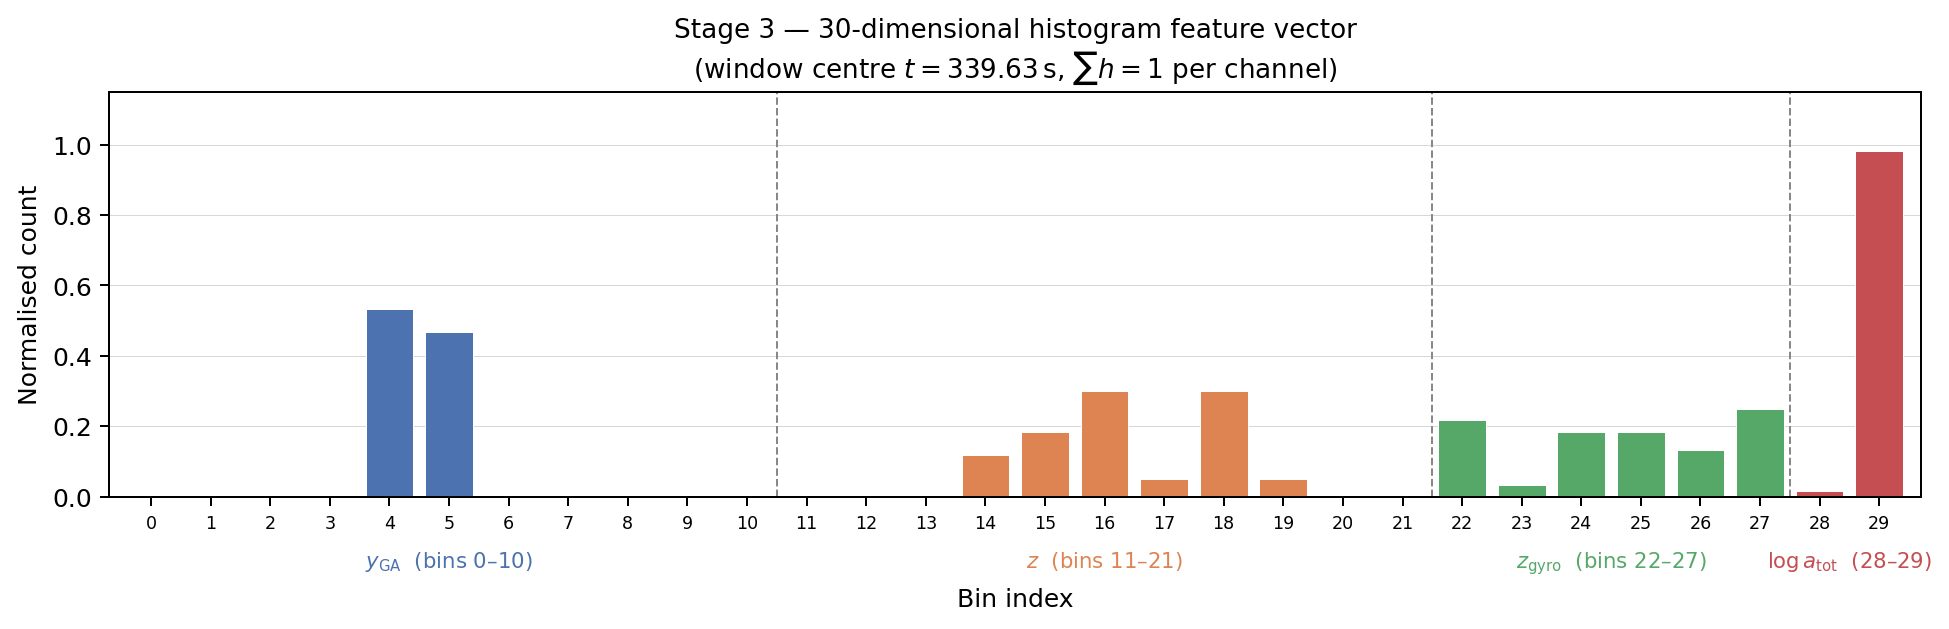
\includegraphics[width=\textwidth]{figures/data_stages_example.png}
\caption{Stage~3 — 30-dimensional normalised histogram feature vector for the
300\,ms window centred at $t=339.63$\,s. Each colour corresponds to one sensor
channel; dashed lines mark channel boundaries. The $y_{\mathrm{GA}}$ channel
splits across bins~4--5, indicating the mouse posture oscillated near the
boundary between two ranges during this window. The $z$ channel shows a
bimodal pattern (bins~16 and~18), and all six $z_{\mathrm{gyro}}$ bins are
occupied, reflecting varied angular velocity. Each channel sums to~1.}
\label{fig:stage3}
\end{figure}

\FloatBarrier
\section{CDF Transformation and EMD Distance}

\subsection{CDF Representation}

Earth Mover's Distance measures how much ``probability mass'' must be moved to transform one distribution into another~\cite{rubner2000}. In one dimension, Wasserstein-1 distance between two normalized histograms can be computed efficiently as the L1 distance between their cumulative distribution functions (CDFs).

For each channel $c$, define the CDF of window $i$ as:

\begin{equation}
    H_{i,c,b} = \sum_{r=1}^{b} h_{i,c,r}.
\end{equation}

The Python code additionally divides the CDF L1 sum by $(B_c - 1)$, where $B_c$ is the number of bins for channel $c$. This gives each channel comparable weight even when it has a different number of bins.

\subsection{Per-Channel EMD Approximation}

For two windows $i$ and $j$, the per-channel CDF distance is:

\begin{equation}
    d_c(i,j) =
    \frac{1}{B_c - 1}
    \sum_{b=1}^{B_c}
    \left| H_{i,c,b} - H_{j,c,b} \right|.
\end{equation}

This is the one-dimensional Wasserstein/EMD distance for uniformly spaced bins, up to the normalization used in the implementation.

\subsection{Total Behavioral Distance}

The total distance between two behavioral windows is the sum across channels:

\begin{equation}
    d(i,j) = \sum_{c=1}^{4} d_c(i,j).
\end{equation}

In code, the four per-channel CDF vectors are concatenated into a single feature vector $\mathbf{C}_i \in \mathbb{R}^{30}$, so the total distance reduces to a single L1 call:

\begin{equation}
    d(i,j) = \left\| \mathbf{C}_i - \mathbf{C}_j \right\|_1.
\end{equation}

The per-channel normalization by $(B_c - 1)$ is absorbed into the concatenated representation, so the single L1 call correctly weights all four channels.

\begin{figure}[h]
\centering
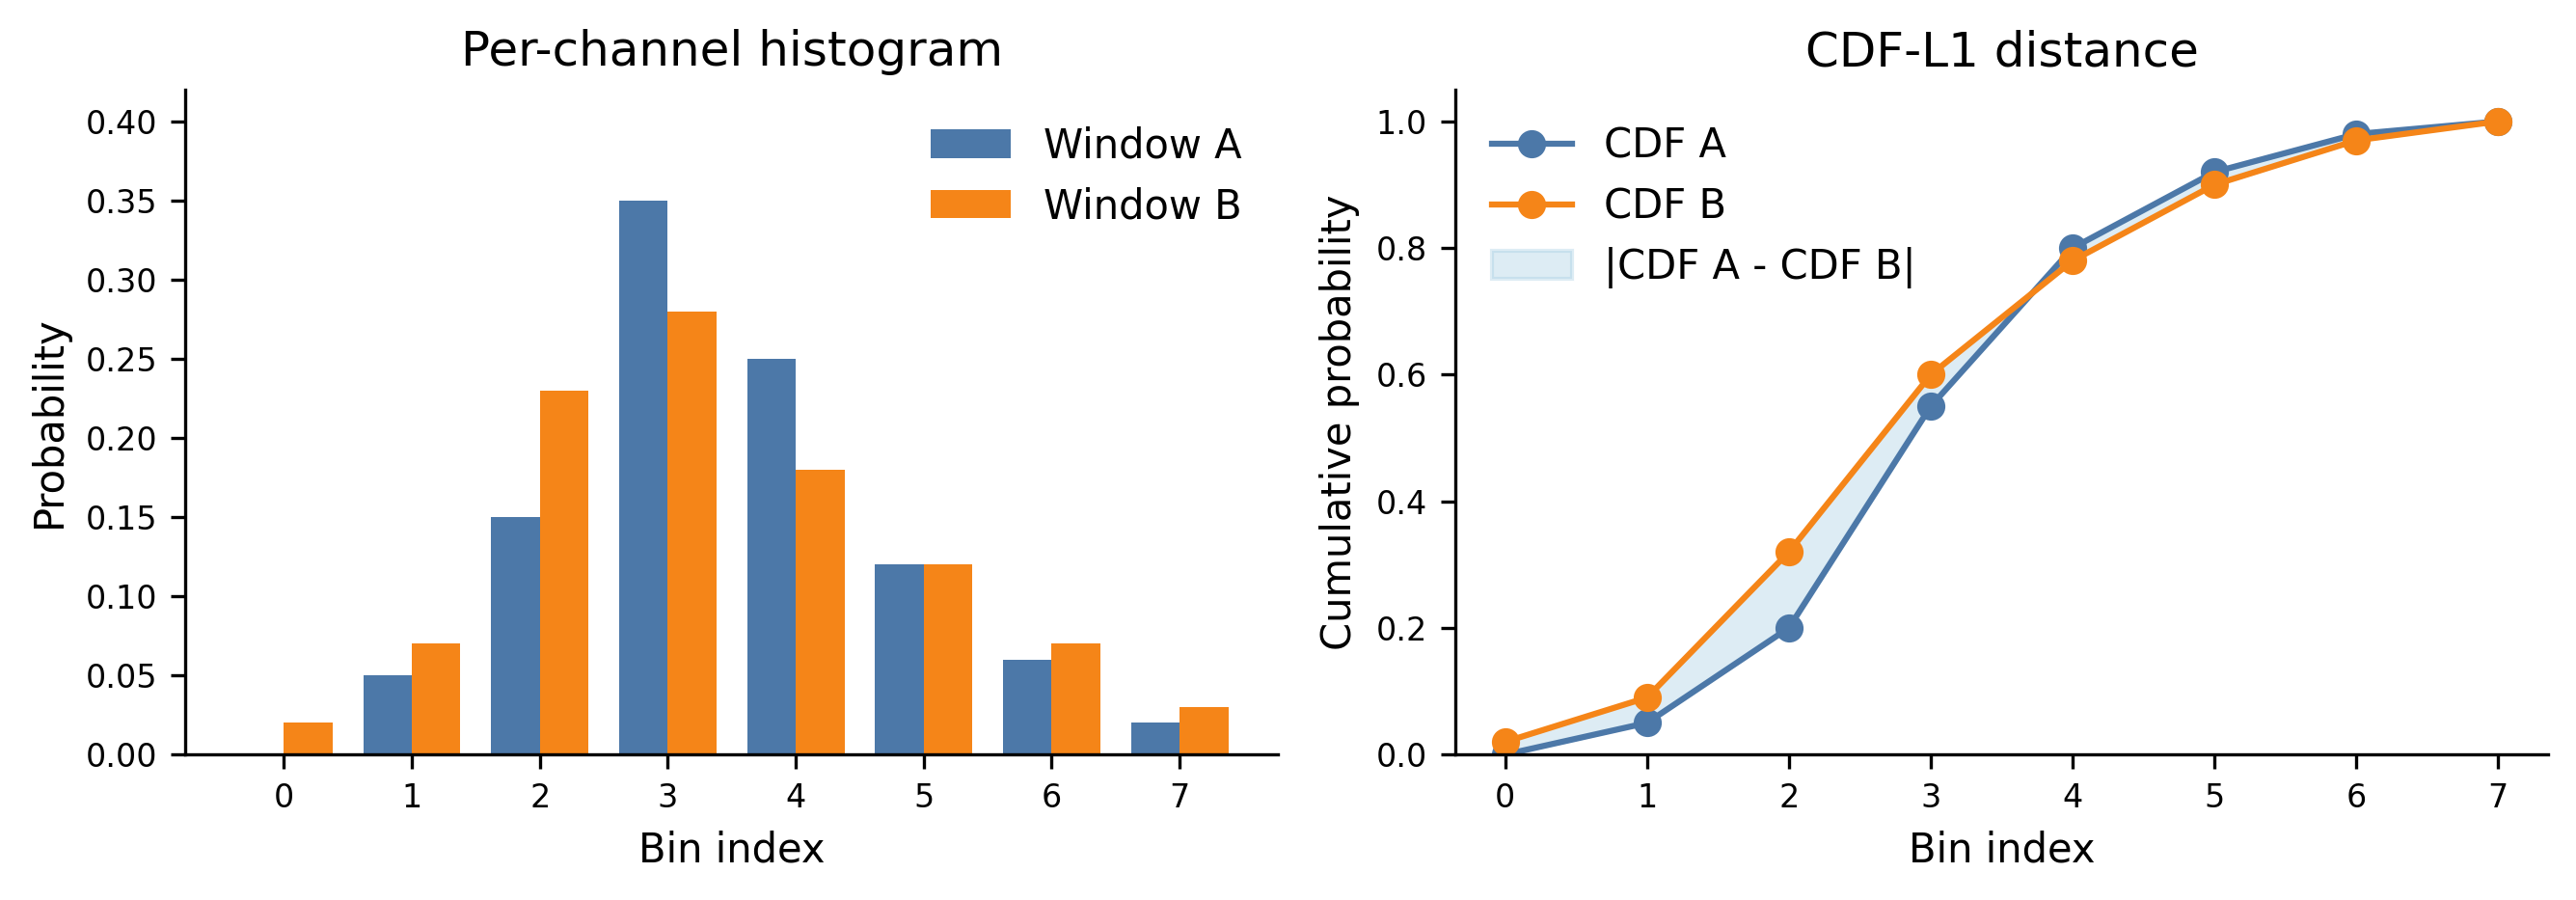
\includegraphics[width=0.9\textwidth]{figures/histogram_cdf_example.png}
\caption{Toy example showing how two window-level histograms are transformed into CDFs. In one dimension, the L1 area between CDFs gives the Wasserstein/EMD distance used by the clustering methods.}
\label{fig:hist-cdf}
\end{figure}

\subsection{AP Similarity}

Affinity Propagation requires similarities rather than distances. The MATLAB pipeline uses negative squared EMD similarity:

\begin{equation}
    s(i,j) = -d(i,j)^2.
\end{equation}

The Python AP methods follow the same similarity convention, but the preference setting depends on the AP variant. For full AP, the preference is set to:

\begin{equation}
    p = \min_{i,j} s(i,j),
\end{equation}

matching the current MATLAB setting \texttt{param = min(s(:,3))} in \texttt{VPAPPAxes.m}, where column~3 of \texttt{s} stores the pairwise similarity values. For random-sampled AP, coreset AP, sparse AP, k-means-sampled AP, and stratified AP, the code estimates the same global minimum similarity by sampling 500,000 random pairs from all $N$ windows. Two-level AP is the main exception: it uses median affinity within local blocks and again among candidate exemplars, because a global minimum preference is too conservative at those smaller local scales.

\FloatBarrier
\section{Role of FAISS}

FAISS~\cite{johnson2021} is not itself the behavioral clustering algorithm in this pipeline. It is used as a fast nearest-neighbor engine operating on the CDF feature vectors computed in the previous section. In the AP sampled, coreset, k-means sampled, stratified, sparse, and two-level methods, AP finds a smaller set of exemplars. FAISS then answers:

\begin{center}
\emph{For this window, which exemplar has the smallest CDF-L1 distance?}
\end{center}

Mathematically, if $\mathcal{E} = \{\mathbf{e}_1,\ldots,\mathbf{e}_K\}$ is the final exemplar set, every window $i$ receives label:

\begin{equation}
    \ell_i = \arg\min_{k \in \{1,\ldots,K\}}
    \left\| \mathbf{C}_i - \mathbf{e}_k \right\|_1.
\end{equation}

Thus FAISS accelerates assignment and KNN graph construction; it does not replace AP's exemplar selection.

\begin{figure}[h]
\centering
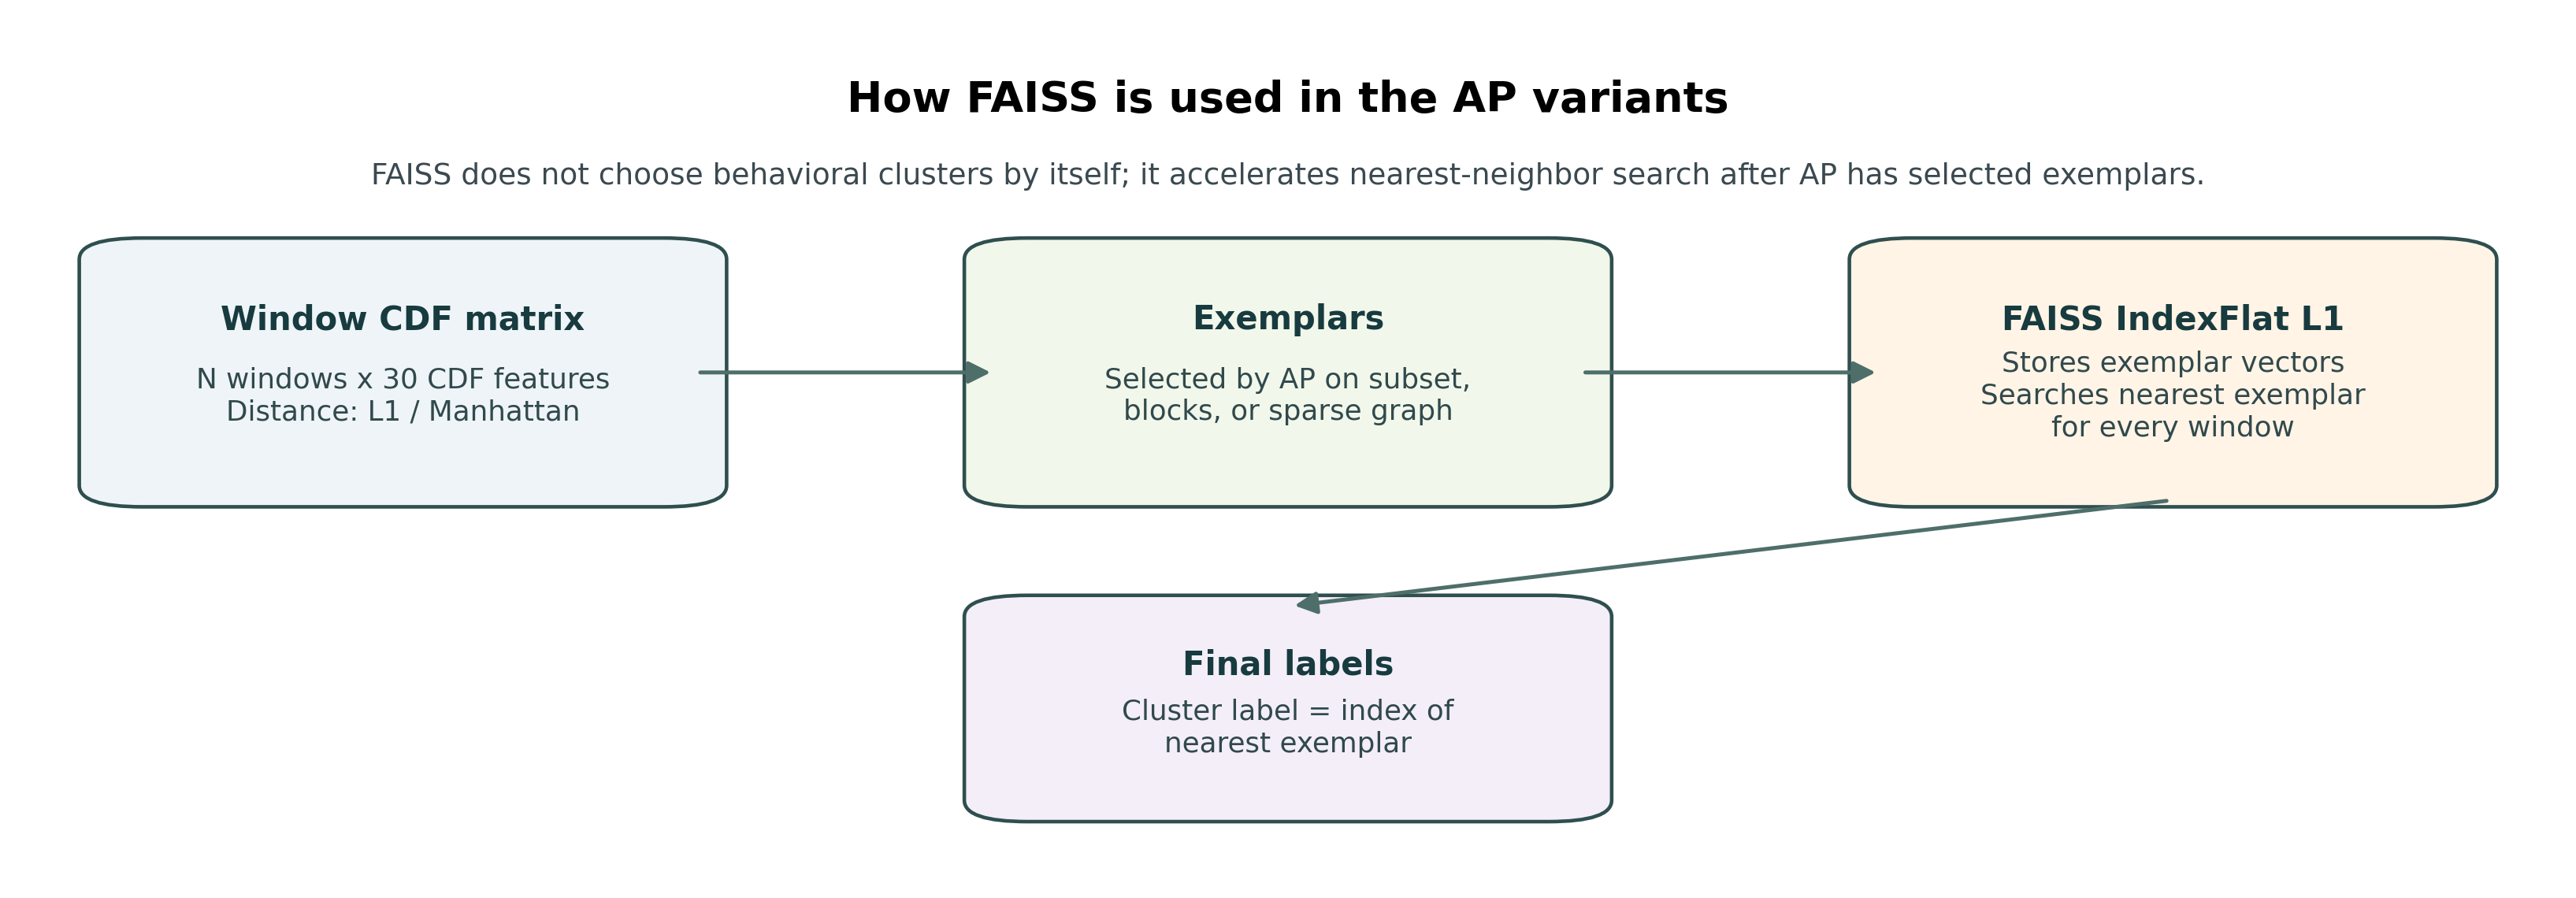
\includegraphics[width=\textwidth]{figures/faiss_usage.png}
\caption{FAISS usage in the AP variants. AP selects exemplars; FAISS stores those exemplar vectors and performs fast nearest-neighbor search under L1 distance to assign every window to its closest exemplar.}
\label{fig:faiss-usage}
\end{figure}

\FloatBarrier
\section{Why the Python Pipeline Is Faster Than the MATLAB-Style Approach}

The speed improvement comes from two separate changes. First, the distance computation is vectorized: each window is represented as a CDF vector, and the EMD-like distance between two windows is computed by a simple L1 distance between CDF vectors. This avoids repeatedly calling a MATLAB/MEX EMD routine inside nested loops.

Second, the scalable AP variants avoid constructing the full dense $N \times N$ similarity matrix for large datasets. Full AP is still available as a reference method, but the scalable methods run AP on a subset, on local blocks, or on a sparse KNN graph, then use FAISS to assign all windows to the final exemplars. The assignment step scales with the number of windows times the number of exemplars rather than all pairs of windows.

\begin{figure}[h]
\centering
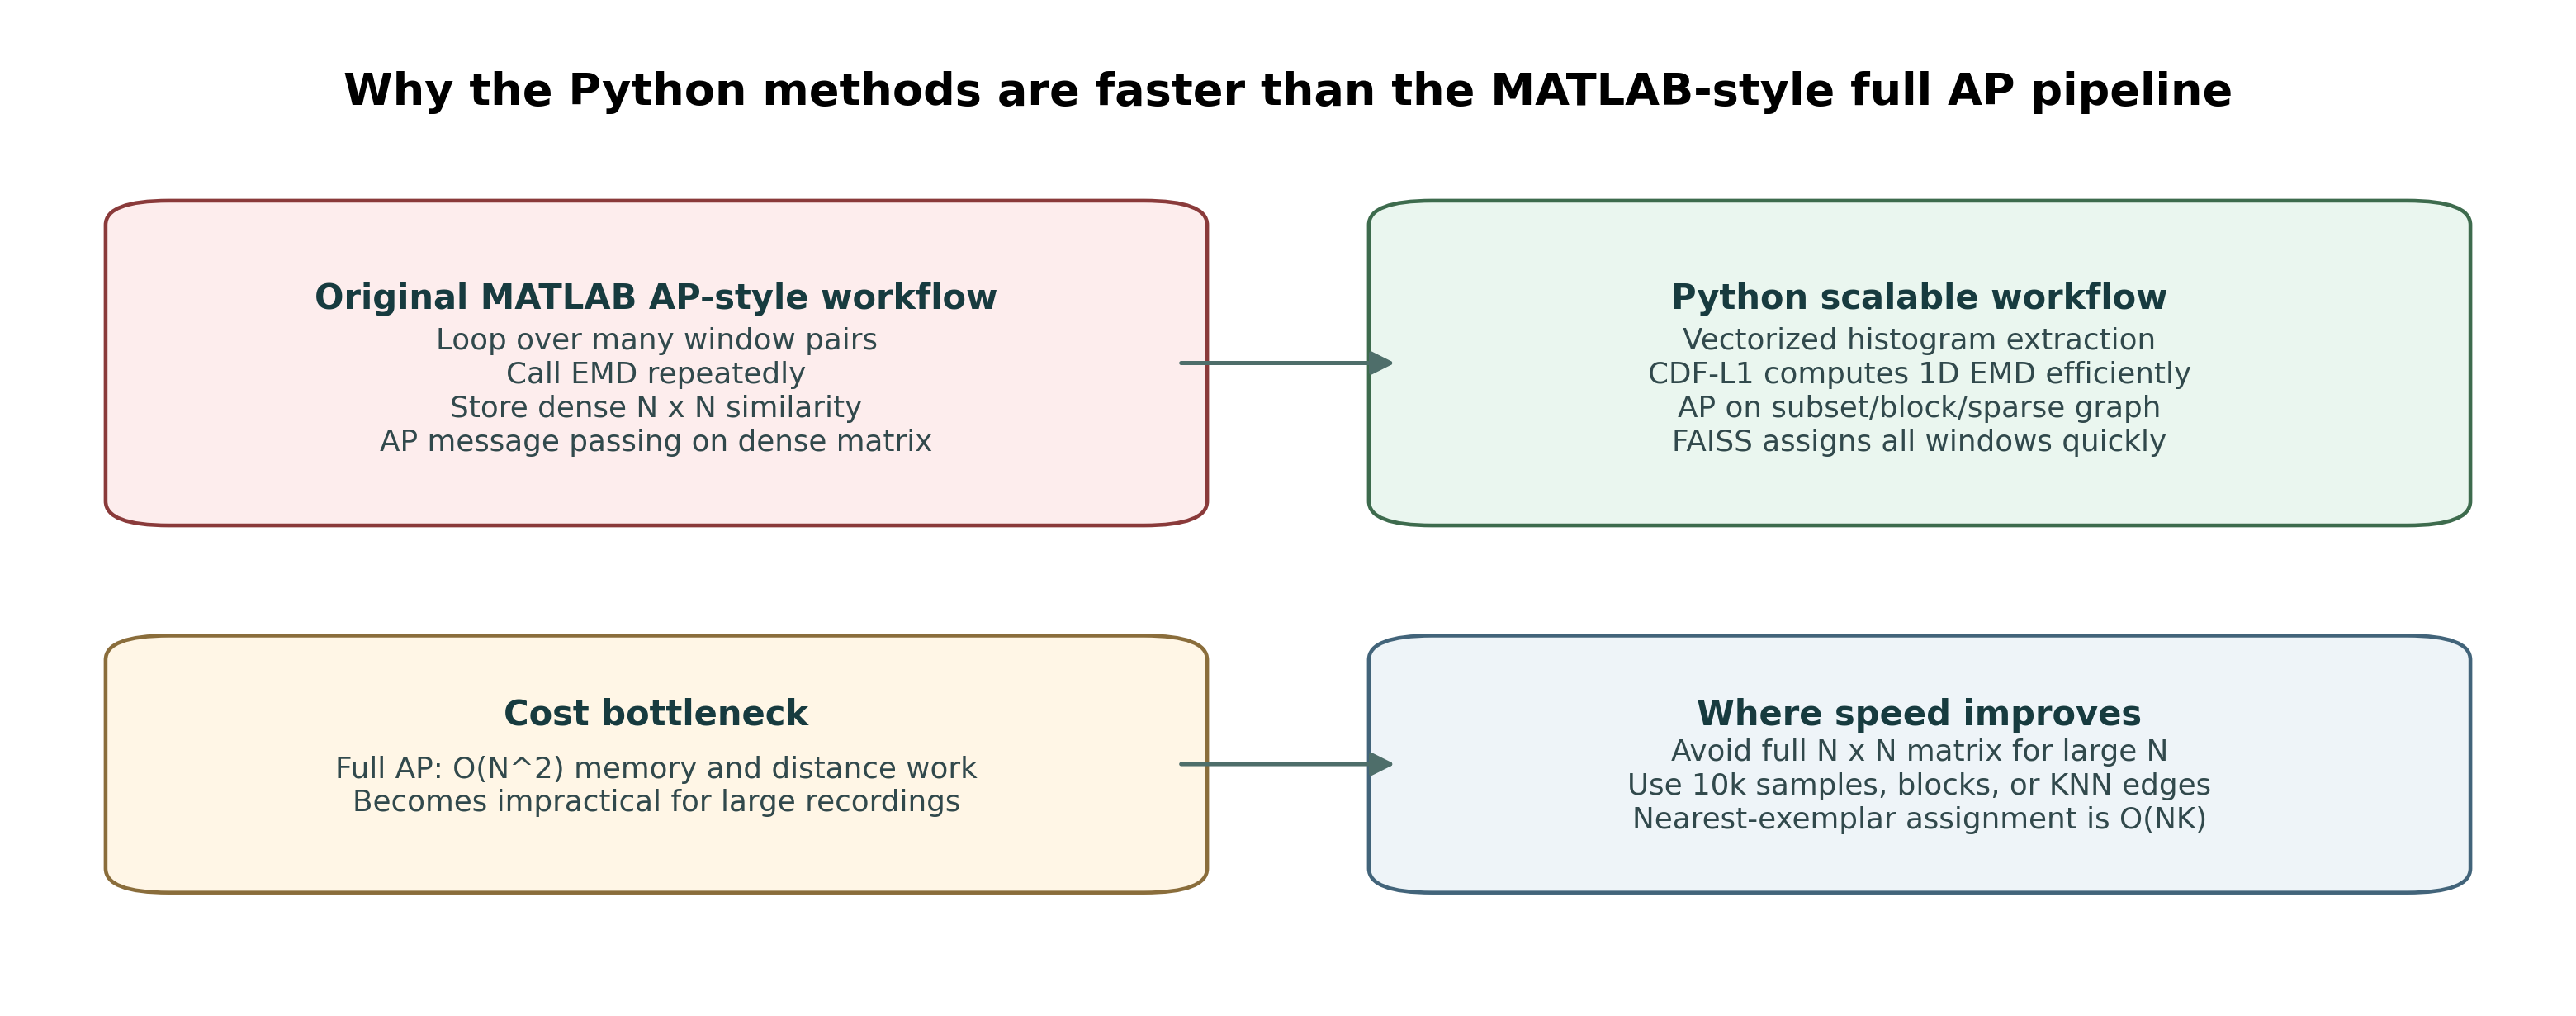
\includegraphics[width=\textwidth]{figures/matlab_python_speed.png}
\caption{Main computational differences between the MATLAB-style full AP workflow and the scalable Python variants. The largest gain comes from avoiding dense all-pairs AP computations when $N$ is large.}
\label{fig:matlab-python-speed}
\end{figure}

\FloatBarrier
\section{Affinity Propagation Algorithm}
\label{sec:ap-algorithm}

Affinity Propagation (AP)~\cite{frey2007} is an exemplar-based clustering algorithm. Rather than requiring the number of clusters to be specified in advance, AP discovers exemplars --- representative data points that best summarize groups of similar points --- by iteratively passing messages between all pairs of points until a consistent set of exemplars emerges.

\subsection{Problem Formulation}

Given $N$ data points with a pairwise similarity matrix $S \in \mathbb{R}^{N \times N}$, AP seeks a subset $\mathcal{E}$ of exemplars and an assignment $e_i \in \mathcal{E}$ for each point $i$ that maximizes the total similarity:

\begin{equation}
    \mathcal{E}^* = \arg\max_{\mathcal{E}} \sum_{i=1}^{N} s(i,\, e_i),
\end{equation}

subject to the self-consistency constraint that every exemplar must represent itself:
\begin{equation}
    e_k = k \quad \text{for all } k \in \mathcal{E}.
\end{equation}

In the current pipeline, the similarity between two windows is the negative squared CDF-L1 distance:
\begin{equation}
    s(i,k) = -d(i,k)^2 = -\left\|\mathbf{C}_i - \mathbf{C}_k\right\|_1^2.
\end{equation}

The diagonal $s(k,k) = p$ is the \textit{preference} parameter, which controls how many exemplars are found. A higher preference (closer to zero) yields more exemplars and therefore more clusters; a lower preference (more negative) yields fewer.

\subsection{Message-Passing Equations}

AP maintains two $N \times N$ message matrices that are updated alternately at each iteration.

\paragraph{Responsibility $r(i,k)$.}
The responsibility $r(i,k)$ is sent from point $i$ to candidate exemplar $k$. It reflects how much point $i$ ``prefers'' $k$ as its exemplar relative to all other candidates:

\begin{equation}
    r(i,k) \;\leftarrow\; s(i,k) - \max_{k' \neq k}\bigl\{a(i,k') + s(i,k')\bigr\}.
\end{equation}

A large positive $r(i,k)$ means $k$ is a better candidate for $i$ than any alternative.

\paragraph{Availability $a(i,k)$.}
The availability $a(i,k)$ is sent from candidate exemplar $k$ to point $i$. It reflects how ``willing'' $k$ is to be an exemplar, given the support it receives from other points.

For off-diagonal entries ($i \neq k$):
\begin{equation}
    a(i,k) \;\leftarrow\; \min\!\left(0,\;\; r(k,k) + \sum_{i' \notin \{i,\,k\}} \max\!\bigl(0,\, r(i',k)\bigr)\right).
\end{equation}

The minimum with zero enforces that only already-supported candidates can attract more points. For the self-availability ($i = k$):
\begin{equation}
    a(k,k) \;\leftarrow\; \sum_{i' \neq k} \max\!\bigl(0,\, r(i',k)\bigr).
\end{equation}

\paragraph{Damping.}
To prevent numerical oscillations during message passing, each new message is mixed with its previous value using damping factor $\lambda \in [0.5, 1)$:
\begin{align}
    r &\;\leftarrow\; (1-\lambda)\,r_{\mathrm{new}} + \lambda\,r_{\mathrm{old}}, \\
    a &\;\leftarrow\; (1-\lambda)\,a_{\mathrm{new}} + \lambda\,a_{\mathrm{old}}.
\end{align}

The current pipeline uses $\lambda = 0.9$ for all AP variants (both the scikit-learn calls and the custom sparse AP implementation). This is higher than the scikit-learn default of 0.5, and was chosen to improve convergence stability on the high-dimensional CDF feature space.

\subsection{Convergence and Assignment}

At each iteration, exemplars are identified by checking the diagonal of $R + A$. Point $k$ is an exemplar when:
\begin{equation}
    r(k,k) + a(k,k) > 0.
\end{equation}

The algorithm converges when the set of exemplars remains unchanged for a fixed number of consecutive iterations (default: 15 in scikit-learn) or when the maximum iteration count is reached. After convergence, every point $i$ is assigned to the exemplar that maximises its criterion:
\begin{equation}
    e_i = \arg\max_{k}\;\bigl\{r(i,k) + a(i,k)\bigr\}.
\end{equation}

\subsection{Pseudocode}

Algorithm~\ref{alg:ap} summarizes the full AP procedure.

\begin{algorithm}[h]
\caption{Affinity Propagation}
\label{alg:ap}
\begin{algorithmic}[1]
\Require Similarity matrix $S \in \mathbb{R}^{N \times N}$, preference $p$, damping $\lambda = 0.9$, \texttt{max\_iter} $T = 1000$, \texttt{convergence\_iter} $C = 15$
\Ensure Exemplar set $\mathcal{E}$, assignment labels $\{e_i\}$
\State $S[k,k] \leftarrow p$ \textbf{ for all } $k$ \Comment{set diagonal preference}
\State $R \leftarrow \mathbf{0}_{N\times N}$,\; $A \leftarrow \mathbf{0}_{N\times N}$ \Comment{initialize messages}
\State $\text{stable} \leftarrow 0$
\For{$t = 1$ \textbf{to} $T$}
    \State \textbf{// Update responsibilities}
    \For{each $i$}
        \State $\mathrm{AS}[k] \leftarrow A[i,k] + S[i,k]$ \textbf{ for all } $k$
        \State $R_{\mathrm{new}}[i,k] \leftarrow S[i,k] - \max_{k' \neq k}\,\mathrm{AS}[k']$ \textbf{ for all } $k$
    \EndFor
    \State $R \leftarrow (1-\lambda)\,R_{\mathrm{new}} + \lambda\,R$
    \State \textbf{// Update availabilities}
    \For{each $k$}
        \State $\mathrm{Rp}[i'] \leftarrow \max(0,\, R[i',k])$ \textbf{ for all } $i' \neq k$
        \State $A_{\mathrm{new}}[i,k] \leftarrow \min\!\bigl(0,\; R[k,k] + \sum_{i' \notin \{i,k\}} \mathrm{Rp}[i']\bigr)$ \textbf{ for all } $i \neq k$
        \State $A_{\mathrm{new}}[k,k] \leftarrow \sum_{i' \neq k} \mathrm{Rp}[i']$
    \EndFor
    \State $A \leftarrow (1-\lambda)\,A_{\mathrm{new}} + \lambda\,A$
    \State \textbf{// Check convergence}
    \State $\mathcal{E} \leftarrow \{k : R[k,k] + A[k,k] > 0\}$
    \If{$\mathcal{E}$ unchanged from previous iteration}
        \State $\text{stable} \leftarrow \text{stable} + 1$
    \Else
        \State $\text{stable} \leftarrow 0$
    \EndIf
    \If{$\text{stable} \geq C$} \textbf{break} \EndIf
\EndFor
\State $e_i \leftarrow \arg\max_k\,\{R[i,k] + A[i,k]\}$ \textbf{ for all } $i$ \Comment{final assignment}
\State \Return $\mathcal{E}$, $\{e_i\}$
\end{algorithmic}
\end{algorithm}

\subsection{Time and Memory Complexity}

Full AP requires storing and updating two $N \times N$ message matrices, giving:

\begin{center}
\begin{tabular}{ll}
\toprule
Resource & Cost \\
\midrule
Memory & $O(N^2)$ \\
Time per iteration & $O(N^2)$ \\
Total time & $O(T \cdot N^2)$ \\
\bottomrule
\end{tabular}
\end{center}

For $N = 25{,}000$ and $T \approx 200$ iterations, full AP requires approximately 18\,GB of memory and several minutes of compute. This is the fundamental bottleneck that motivates all scalable AP variants described in Section~\ref{sec:clustering-methods}.

\subsection{Parameter Settings Used in This Pipeline}

Table~\ref{tab:ap-params} lists the AP hyperparameters used across all variants in the current implementation.

\begin{table}[h]
\centering
\caption{AP hyperparameter settings used in the current pipeline. Two-level AP uses different iteration limits at each level because block-level AP operates on smaller subproblems.}
\label{tab:ap-params}
\begin{tabular}{lcccp{4.2cm}}
\toprule
Method & $\lambda$ & \texttt{max\_iter} & \texttt{conv\_iter} & Preference \\
\midrule
AP Full            & 0.9 & 1000 & 15 & exact $\min$ of $N{\times}N$ affinity \\
AP Sampled         & 0.9 & 1000 & 15 & global min$^\dagger$ \\
AP Coreset         & 0.9 & 1000 & 15 & global min$^\dagger$ \\
AP K-Means         & 0.9 & 1000 & 15 & global min$^\dagger$ \\
AP Stratified      & 0.9 & 1000 & 15 & global min$^\dagger$ \\
AP Sparse (custom, $K=1000$) & 0.9 & 1000 & 15 & global min$^\dagger$ \\
AP Two-level (L1)  & 0.9 & 300  & 15 & per-block median affinity \\
AP Two-level (L2)  & 0.9 & 500  & 30 & median among candidate exemplars \\
\bottomrule
\multicolumn{5}{l}{$^\dagger$ Estimated from 500,000 random pairs drawn from all $N$ windows.}
\end{tabular}
\end{table}

All variants use $\lambda = 0.9$, which is higher than the scikit-learn default of 0.5. A higher damping value slows convergence but reduces oscillation, which improves stability when running AP on high-dimensional CDF feature vectors.

\FloatBarrier
\section{Clustering Methods}
\label{sec:clustering-methods}

The current comparison script evaluates seven AP-family methods plus one HDBSCAN reference method. AP methods produce cluster exemplars; HDBSCAN identifies dense regions and may label sparse points as noise.

\begin{figure}[h]
\centering
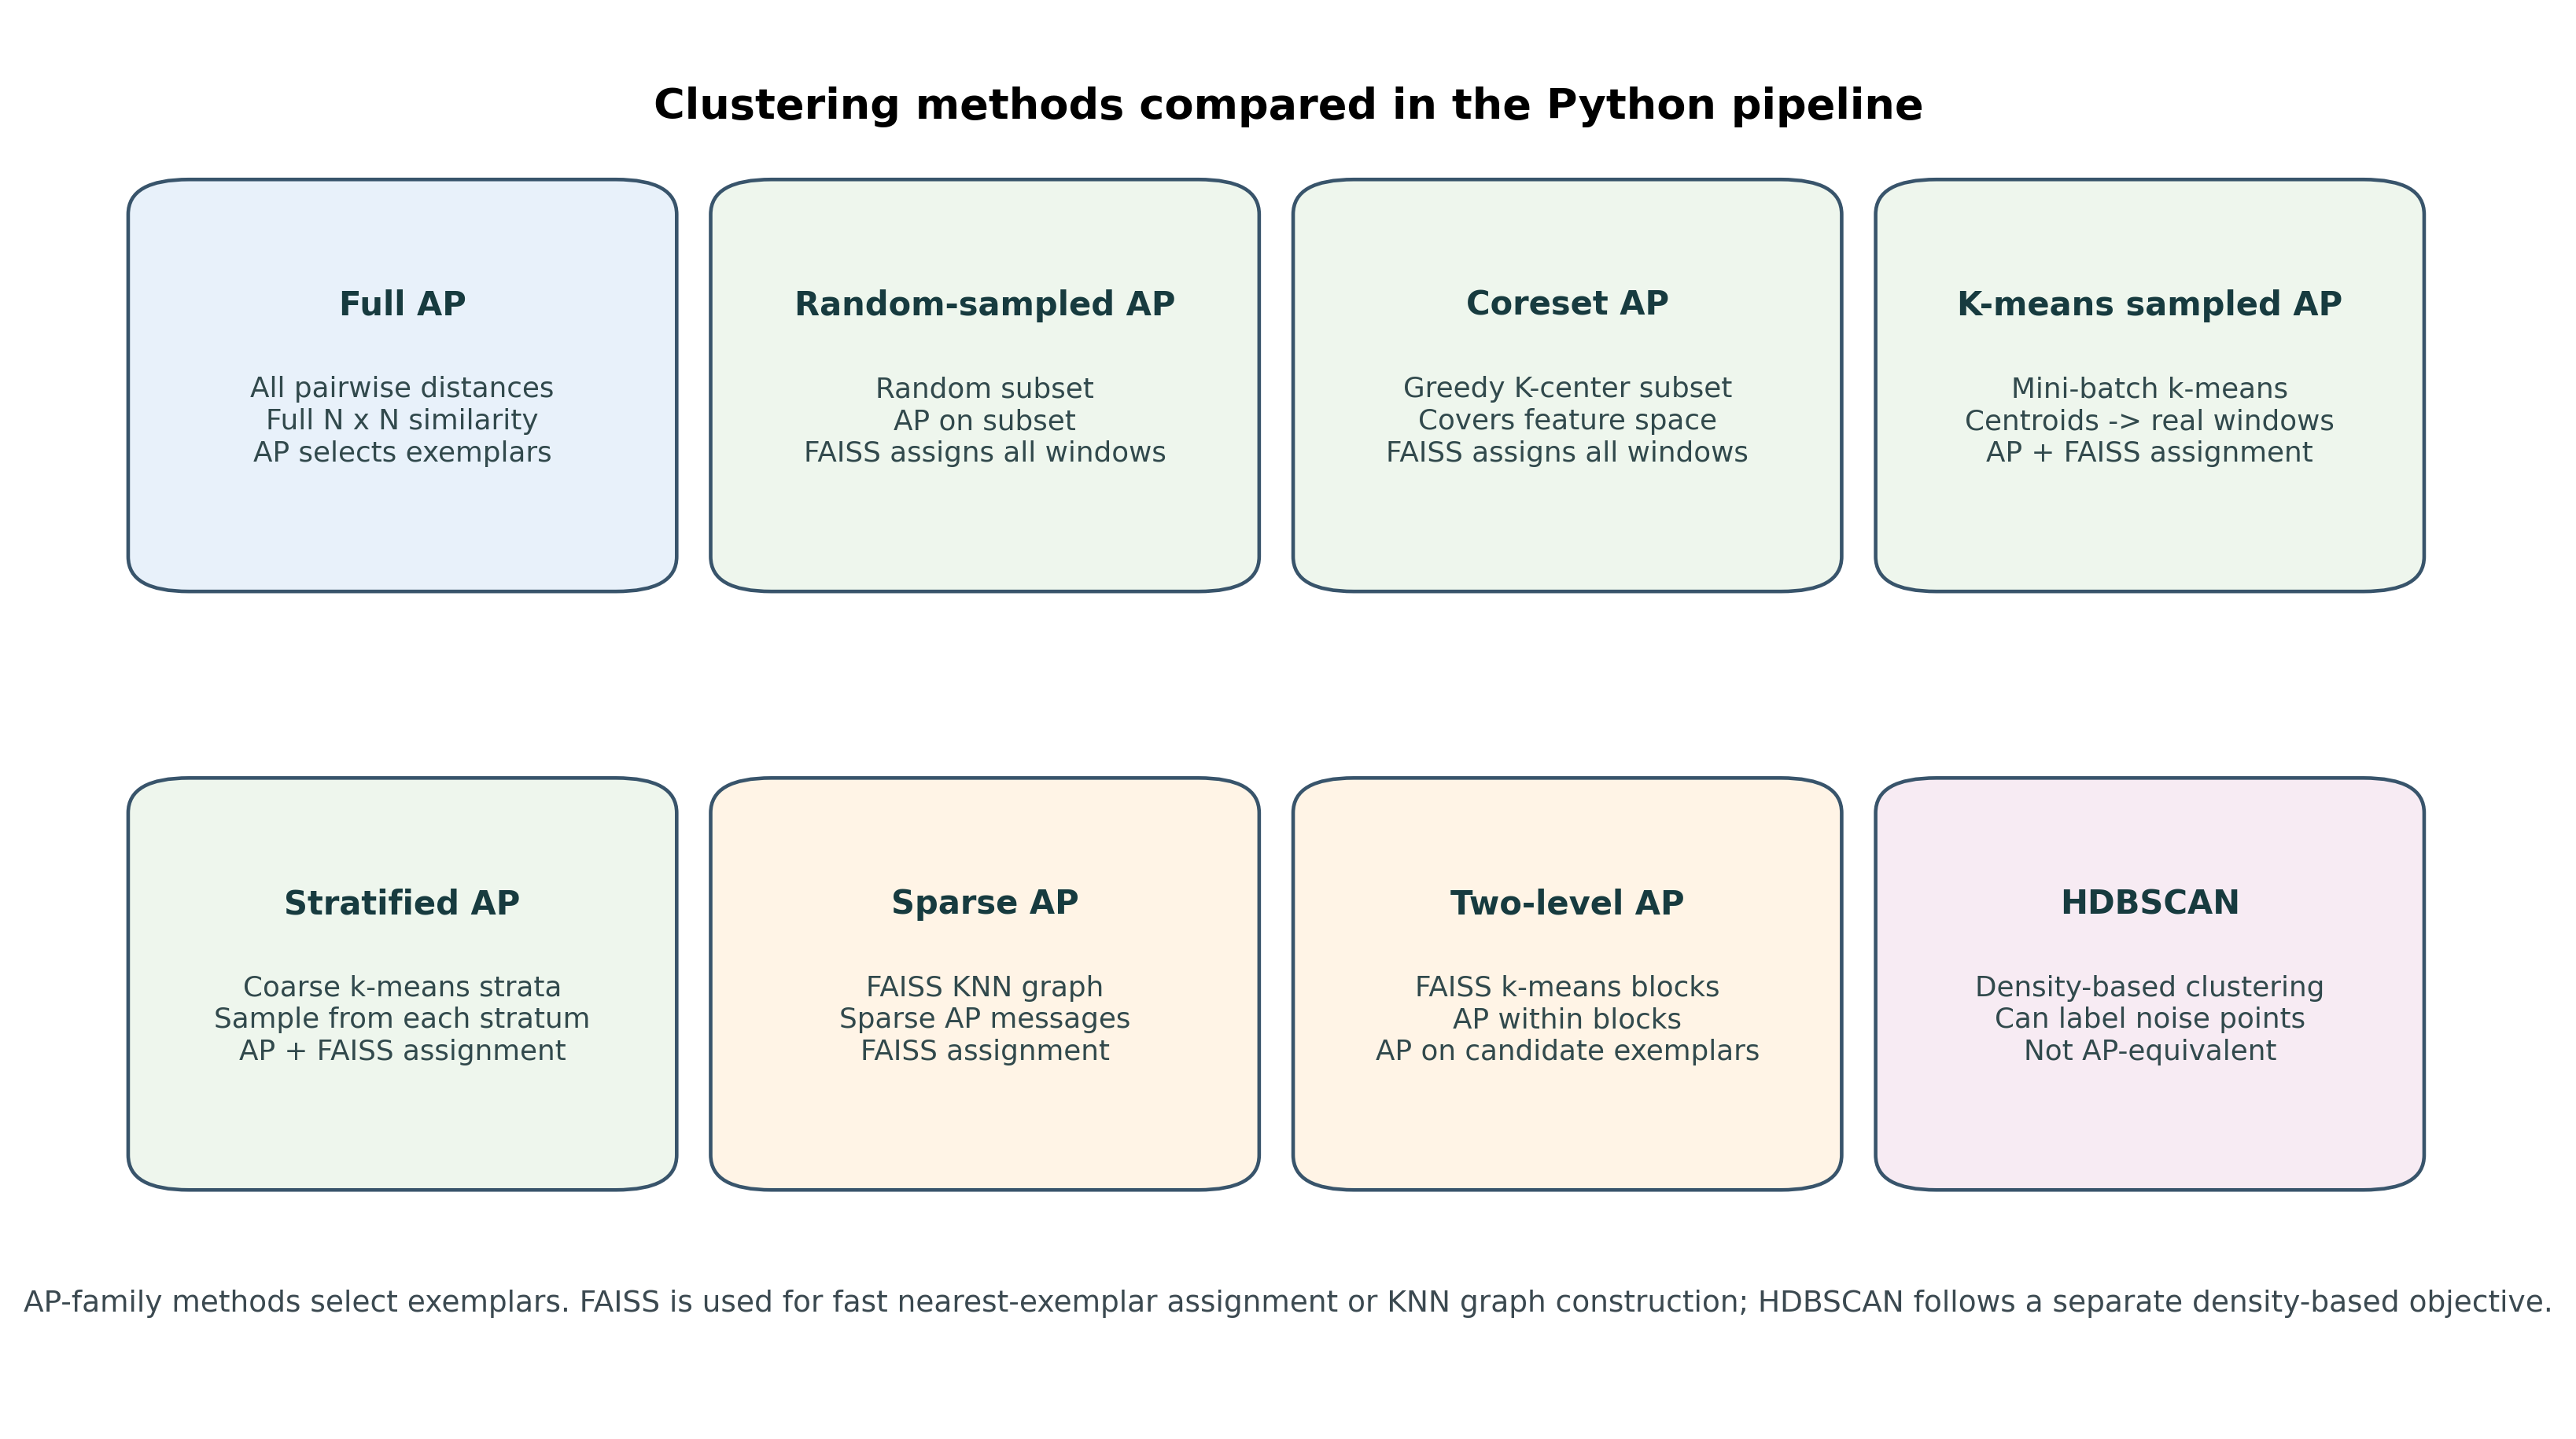
\includegraphics[width=\textwidth]{figures/method_overview.png}
\caption{Visual summary of the clustering methods currently compared in \texttt{Python\_Pipeline}. The AP-family methods differ mainly in how they reduce the cost of exemplar selection before assigning all windows to final exemplars.}
\label{fig:method-overview}
\end{figure}

\subsection{Full Affinity Propagation}

Full AP~\cite{frey2007} is the closest Python equivalent to the MATLAB algorithm. It computes the full pairwise distance matrix:

\begin{equation}
    D \in \mathbb{R}^{N \times N},
\end{equation}

converts it to a similarity matrix $S = -D^2$, fills the diagonal with the AP preference, and runs scikit-learn's~\cite{pedregosa2011} \texttt{AffinityPropagation} with precomputed affinities. The preference is set to the exact minimum of the $N{\times}N$ affinity matrix, matching the MATLAB \texttt{AccelCluster} setting. It is the most faithful reference method, but requires $O(N^2)$ memory and $O(N^2)$ work per AP iteration, so it is skipped for datasets with $N > 25{,}000$ in the batch comparison.

\subsection{Random-Sampled AP}

Random-sampled AP reduces the AP cost by selecting a subset of windows:

\begin{enumerate}
    \item Randomly sample \textbf{10,000 windows}.
    \item Run full AP on the sampled windows.
    \item Extract AP exemplars from the sample.
    \item Use FAISS exact L1 search to assign every original window to its nearest exemplar.
\end{enumerate}

The preference is estimated from 500,000 random pairs drawn from \emph{all} $N$ windows (not just the 10,000 sample), keeping the preference scale consistent with full AP. This is the default scalable AP method in the current pipeline.

\subsection{Coreset-Sampled AP}

Coreset-sampled AP replaces random sampling with Greedy K-Center selection. The goal is to select representative windows that cover the feature space, including rare behaviors that random sampling may miss.

\begin{enumerate}
    \item Pick an initial point.
    \item Iteratively add the point farthest from the selected set until \textbf{10,000 windows} are selected.
    \item Run AP on the selected coreset.
    \item Assign all windows to the nearest exemplar using FAISS.
\end{enumerate}

The preference uses the same global min estimate as random-sampled AP (500,000 random pairs from all $N$ windows). This method can improve coverage of rare behavioral modes, but it may not always best match full AP.

\subsection{Sparse AP}

Sparse AP builds a $K$-nearest-neighbor graph over all $N$ windows (FAISS IVFFlat) and runs AP message-passing on that graph rather than on a dense $N \times N$ matrix. The CLI default is $K=100$; the batch comparison in Section~\ref{sec:results} used $K=1{,}000$. Memory drops from $O(N^2)$ to $O(NK)$. The custom message-passing implementation symmetrizes the graph and adds self-loops at the preference value before iterating.

In practice, sparse AP tends to over-fragment: because windows can only communicate with their $K$ nearest neighbours, two behaviorally related windows that happen to sit far apart in feature space may never exchange messages and end up in separate clusters. This is a structural limitation of the approach, not a tuning problem---increasing $K$ helps but requires proportionally more memory.

\subsection{Two-Level AP}

Two-level AP is designed to let all windows participate without forming a global dense affinity matrix.

\begin{enumerate}
    \item Use FAISS k-means to partition all $N$ windows into $M = \max(4,\lfloor N/2500 \rfloor)$ blocks of $\sim$2,500 windows each (FAISS k-means, \texttt{niter}=20).
    \item Run full AP inside each block (\texttt{max\_iter}=300, \texttt{conv\_iter}=15, preference = per-block median affinity) to obtain local candidate exemplars.
    \item Run a second AP over all candidate exemplars $M_{\mathrm{cand}}$ (\texttt{max\_iter}=500, \texttt{conv\_iter}=30, preference = median affinity among candidates).
    \item Assign all windows to the nearest final exemplar using FAISS exact L1 search.
\end{enumerate}

This method reduces AP cost from roughly $O(N^2)$ to approximately $O(N^2/M + M_{\mathrm{cand}}^2)$ over $M$ blocks, where $M_{\mathrm{cand}}$ is the number of candidate exemplars collected from all blocks. The median preference at both levels is an intentional design choice: using the global minimum preference would collapse each local block to a single exemplar, leaving too few candidates for the second-level AP.

\subsection{K-Means-Sampled AP}

K-means-sampled AP uses mini-batch k-means to select central representative windows:

\begin{enumerate}
    \item Run mini-batch k-means with $k = 10{,}000$ to partition all $N$ windows (\texttt{n\_init}=3, \texttt{batch\_size}=$\min(4096, N)$, \texttt{max\_iter}=100).
    \item Map each centroid to the nearest real window using FAISS exact L1 search.
    \item Run AP on the 10,000 selected real windows.
    \item Assign all windows to the nearest AP exemplar using FAISS.
\end{enumerate}

The preference uses the same global min estimate as random-sampled AP (500,000 random pairs from all $N$ windows). Compared with random sampling, this method selects cluster-central rather than boundary points, which can improve ARI against full AP.

\subsection{Stratified-Sampled AP}

Stratified AP first partitions the full dataset into coarse strata and then samples from each stratum.

\begin{enumerate}
    \item Run mini-batch k-means with $k = 200$ coarse strata (\texttt{n\_init}=3, \texttt{batch\_size}=$\min(4096, N)$, \texttt{max\_iter}=100).
    \item Draw approximately equal numbers of windows from each stratum until \textbf{10,000 windows} are selected in total ($\sim$50 per stratum).
    \item Run AP on the stratified sample.
    \item Assign all windows to the nearest exemplar using FAISS.
\end{enumerate}

The preference uses the same global min estimate as random-sampled AP (500,000 random pairs from all $N$ windows). By sampling equally from each stratum, this method ensures that rare behaviors occupying small fractions of the recording are represented in the AP sample, regardless of their frequency.

\subsection{HDBSCAN Reference Method}

HDBSCAN~\cite{campello2013} is included as a density-based reference. It clusters CDF features under L1 distance without needing a preference parameter, and assigns low-density windows a noise label ($-1$) rather than forcing them into a cluster. Reproducing MATLAB AP results is not the goal---HDBSCAN optimises a different objective---but it serves as a useful sanity check and exploratory tool, particularly for identifying whether the recording contains genuinely distinct dense behavioral modes.

\FloatBarrier
\section{Evaluation Metrics}

\subsection{Number of Clusters and Noise}

For AP methods, every window is assigned to a cluster, so the noise percentage is 0\%. For HDBSCAN, some windows may be labeled as noise and are excluded from cluster-size statistics.

\subsection{Silhouette Score}
\label{sec:silhouette}

Silhouette score~\cite{rousseeuw1987} measures how close a point is to its own cluster compared with other clusters. The code computes silhouette using L1 distance on CDF features, subsampling up to 2,000 valid windows for speed. Note that HDBSCAN silhouette scores are not directly comparable to AP-family scores: HDBSCAN may achieve high silhouette by labeling ambiguous boundary windows as noise and retaining only well-separated points, whereas AP assigns every window to a cluster. The interpretation used in the report is:

\begin{center}
\begin{tabular}{ll}
\toprule
Silhouette range & Interpretation \\
\midrule
$>0.5$ & good \\
$0.25$--$0.5$ & reasonable \\
$<0.25$ & poor \\
\bottomrule
\end{tabular}
\end{center}

\subsection{ARI Against Full AP}

Adjusted Rand Index (ARI)~\cite{hubert1985} is used when full AP is available. Full AP is treated as the MATLAB-like reference. ARI is interpreted as:

\begin{center}
\begin{tabular}{ll}
\toprule
ARI value & Meaning \\
\midrule
1 & identical clustering \\
0 & agreement expected by chance \\
$<0$ & worse than chance \\
\bottomrule
\end{tabular}
\end{center}

\FloatBarrier
\section{Datasets}

The current batch comparison evaluates eight datasets.

\begin{table}[h]
\centering
\caption{Datasets included in the current method comparison. Duration is computed as $N \times 300\,\text{ms}$.}
\begin{tabular}{lrrl}
\toprule
Dataset & $N$ & Duration & Description \\
\midrule
\texttt{short\_comparison\_test} & 1,195 & $\sim$6 min & Short subset of comparison\_test for quick testing \\
\texttt{comparison\_test} & 13,799 & $\sim$69 min & Full MATLAB-equivalent reference recording \\
\texttt{mp\_mouse\_1\_jul} & 19,714 & $\sim$99 min & MitoPark Parkinson's mouse, July session \\
\texttt{control\_mouse\_1\_jul} & 23,902 & $\sim$120 min & Control mouse, July session (age-matched) \\
\texttt{control\_mouse\_1\_oct} & 23,906 & $\sim$120 min & Control mouse, October session (age-matched) \\
\texttt{mp\_mouse\_1\_oct} & 23,866 & $\sim$119 min & MitoPark Parkinson's mouse, October session \\
\texttt{still\_test} & 23,877 & $\sim$119 min & Low-motion baseline recording \\
\texttt{moving\_test} & 47,028 & $\sim$235 min & High-motion activity recording \\
\bottomrule
\end{tabular}
\end{table}

\FloatBarrier
\section{Results}
\label{sec:results}

\subsection{Cluster Counts and Silhouette Scores}

Tables~\ref{tab:cluster-counts} and~\ref{tab:silhouette} summarize the current cached comparison results, from a single version-pinned run (\texttt{requirements.txt}; numpy 2.5.2, scikit-learn 1.9.0, faiss-cpu 1.15.0) performed on 2026-08-24. Cluster counts and silhouette scores are shown separately for readability. Full AP is skipped when the dataset has more than 25,000 windows (raised from an earlier 20,000-window threshold after moving to a 48\,GB machine; see the reproducibility note at the end of this section). The accompanying figures use abbreviated axis labels from the plotting code (e.g., \textit{AP twolevel}, \textit{AP kmeans}, \textit{AP stratified}), which correspond to the full method names used in the tables and text.

\begin{figure}[h]
\centering
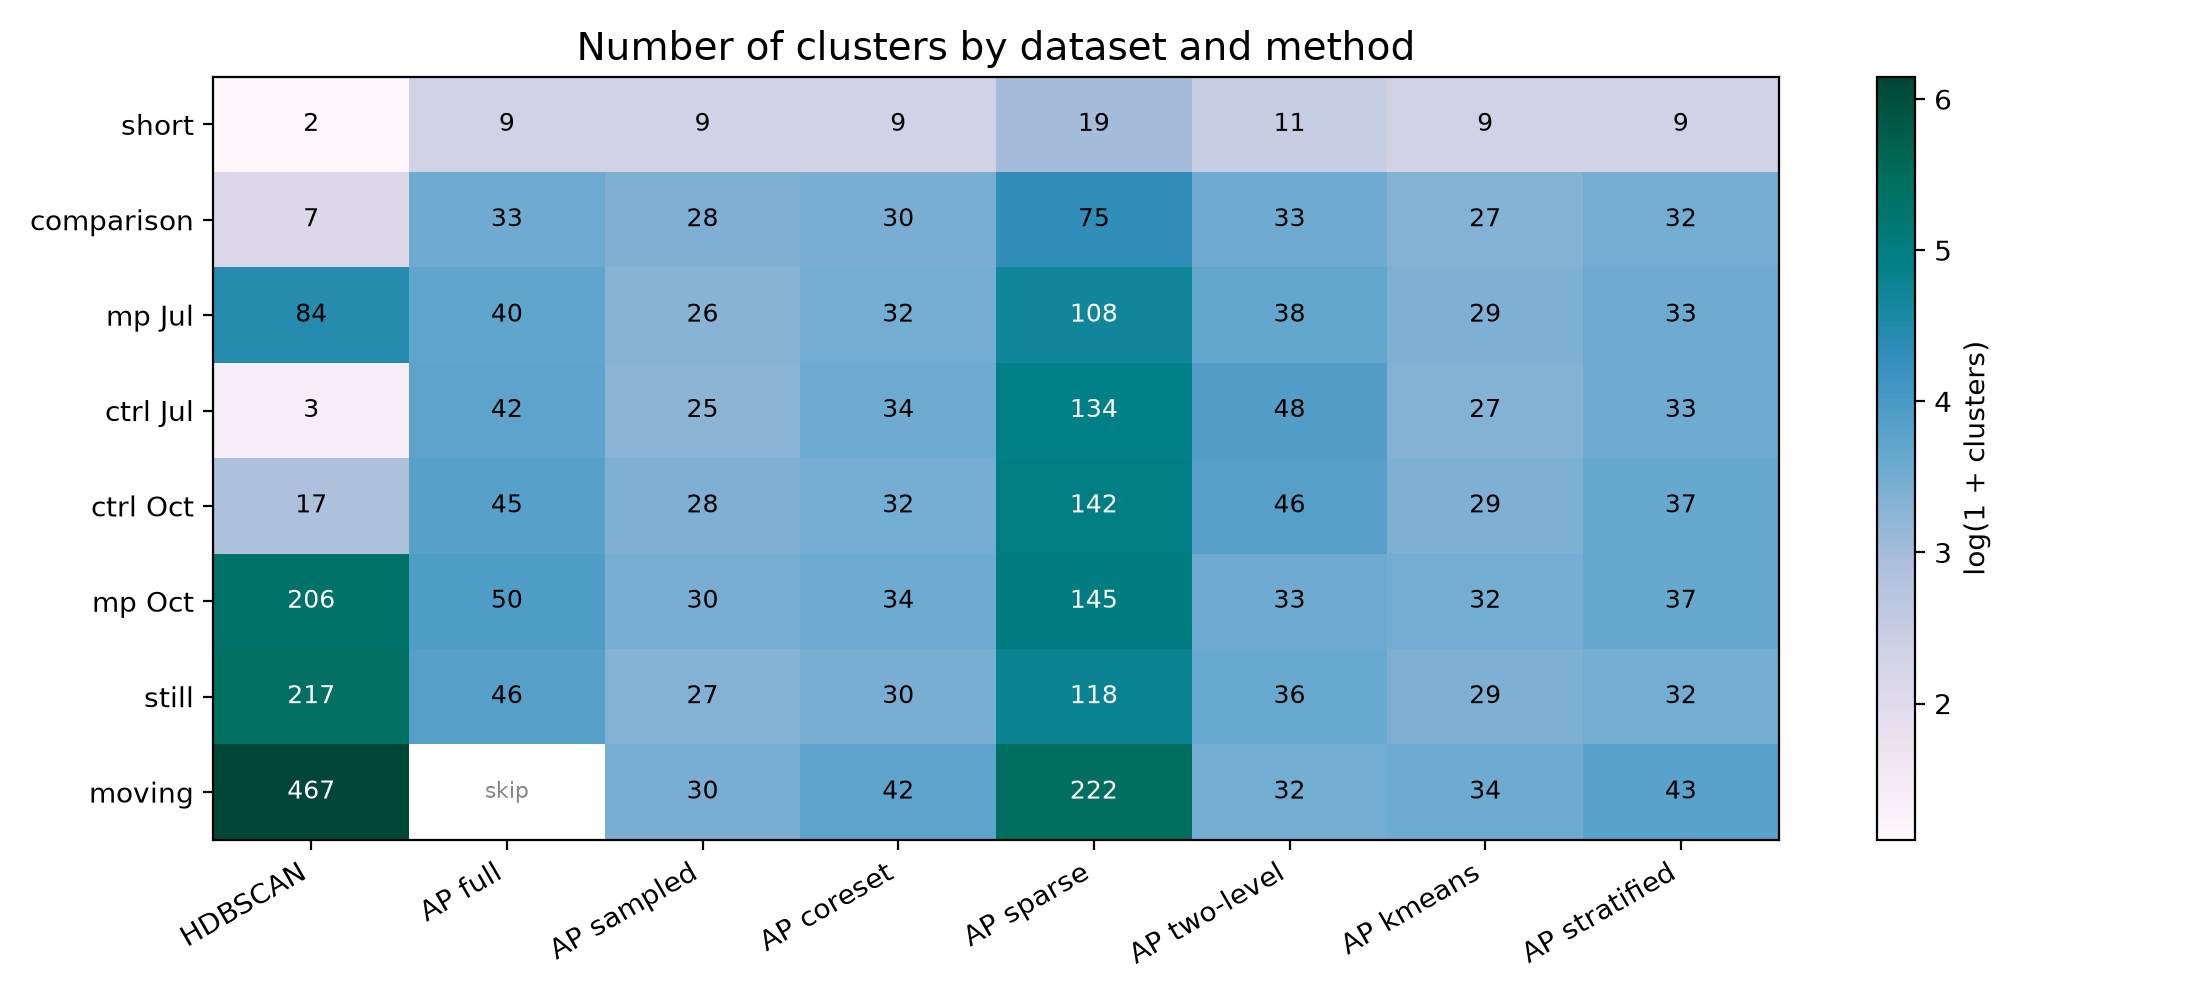
\includegraphics[width=\textwidth]{figures/cluster_count_heatmap.png}
\caption{Heatmap of the number of clusters found by each method. Sparse AP and HDBSCAN tend to produce many more clusters than the AP sampled family.}
\label{fig:cluster-count-heatmap}
\end{figure}

\begin{table}[h]
\centering
\caption{Number of clusters found by each method. A dash indicates that AP Full was skipped because the dataset exceeded the full-AP size threshold. High cluster counts in Sparse AP and HDBSCAN reflect known limitations of those methods rather than desirable results.}
\label{tab:cluster-counts}
\scriptsize
\setlength{\tabcolsep}{5pt}
\begin{tabular}{lcccccccc}
\toprule
Dataset & \rotatebox{90}{\,HDBSCAN\,} & \rotatebox{90}{\,AP Full\,} & \rotatebox{90}{\,AP Sampled\,} & \rotatebox{90}{\,AP Coreset\,} & \rotatebox{90}{\,AP Sparse\,} & \rotatebox{90}{\,AP Two-level\,} & \rotatebox{90}{\,AP K-Means\,} & \rotatebox{90}{\,AP Stratified\,} \\
\midrule
\texttt{short\_comparison\_test} & 2 & 9 & 9 & 9 & 19 & 11 & 9 & 9 \\
\texttt{comparison\_test} & 7 & 33 & 28 & 30 & 75 & 33 & 27 & 32 \\
\texttt{mp\_mouse\_1\_jul} & 84 & 40 & 26 & 32 & 108 & 38 & 29 & 33 \\
\texttt{control\_mouse\_1\_jul} & 3 & 42 & 25 & 34 & 134 & 48 & 27 & 33 \\
\texttt{control\_mouse\_1\_oct} & 17 & 45 & 28 & 32 & 142 & 46 & 29 & 37 \\
\texttt{mp\_mouse\_1\_oct} & 206 & 50 & 30 & 34 & 145 & 33 & 32 & 37 \\
\texttt{still\_test} & 217 & 46 & 27 & 30 & 118 & 36 & 29 & 32 \\
\texttt{moving\_test} & 467 & -- & 30 & 42 & 222 & 32 & 34 & 43 \\
\bottomrule
\end{tabular}
\end{table}

\begin{figure}[h]
\centering
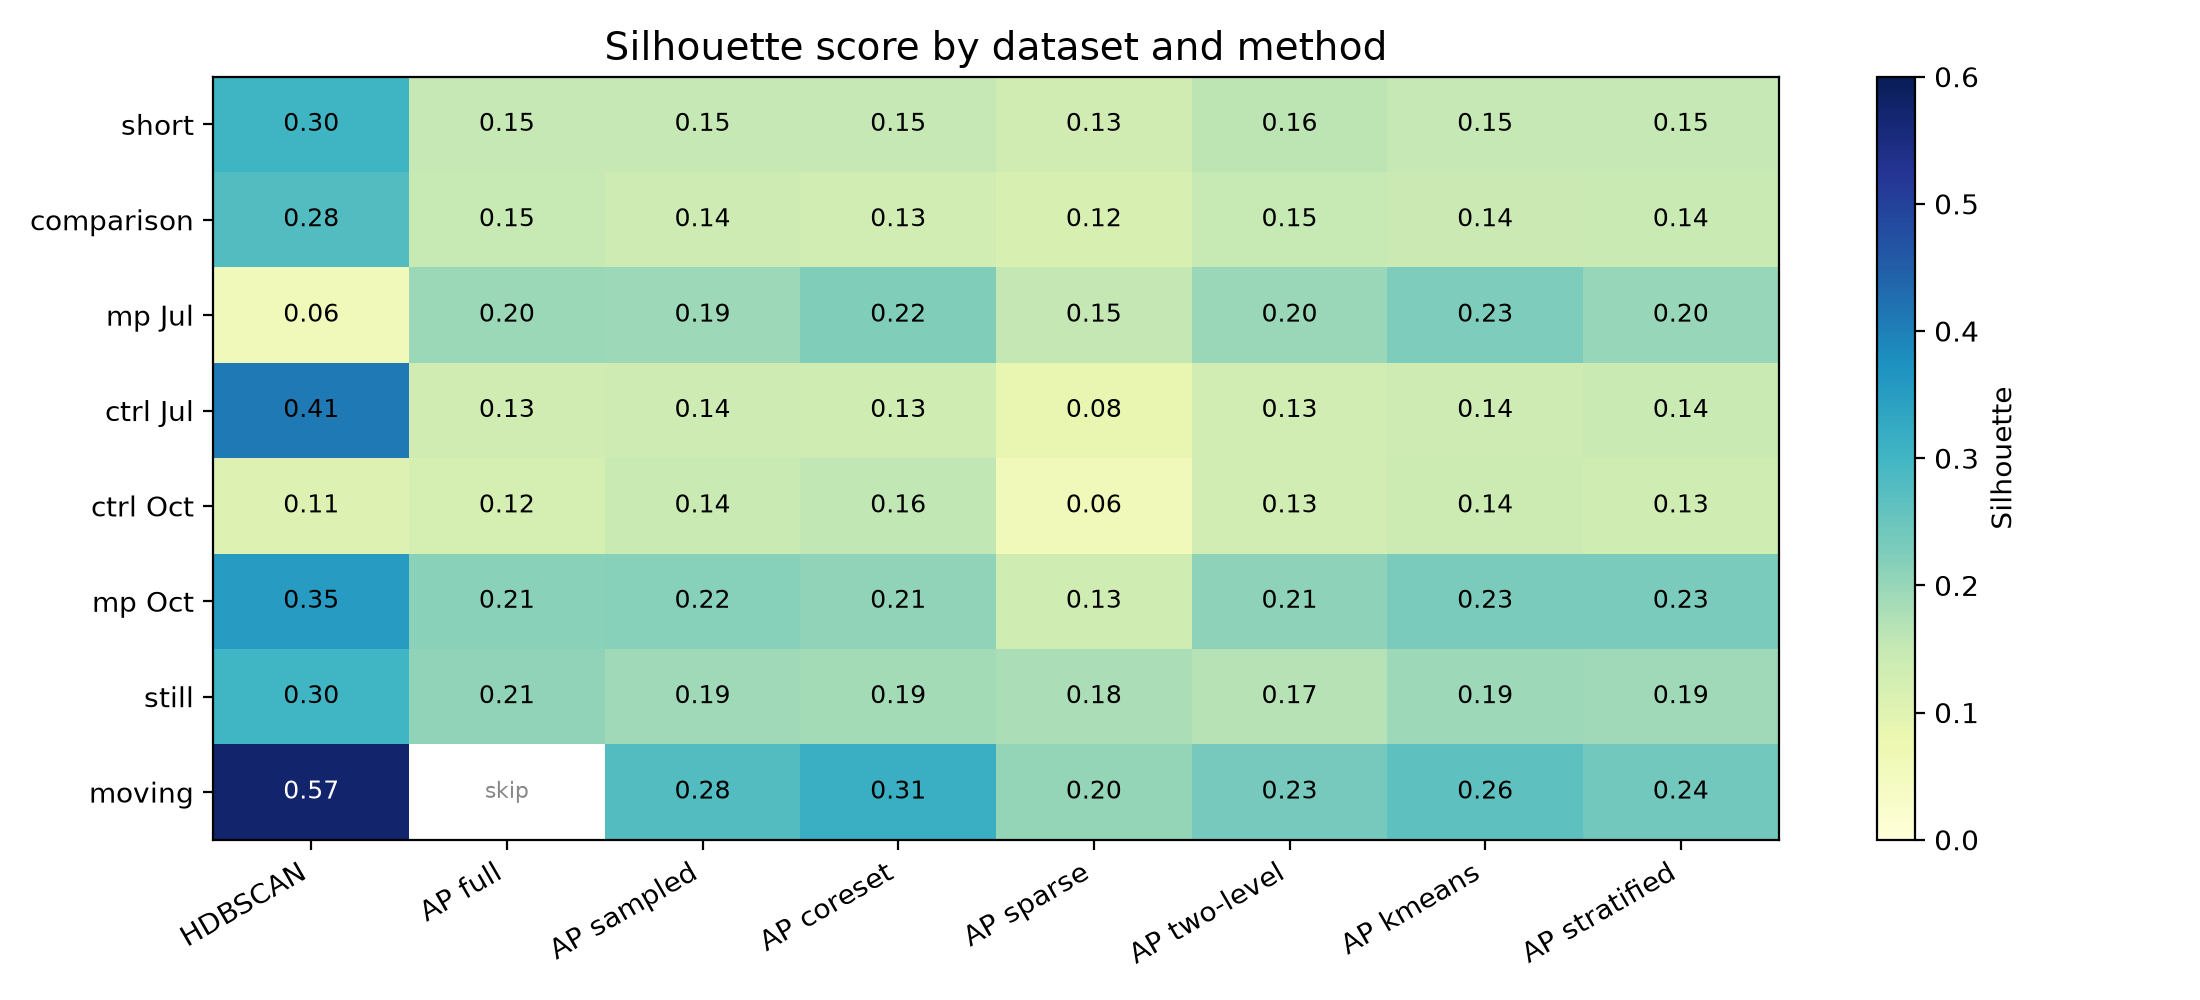
\includegraphics[width=\textwidth]{figures/silhouette_heatmap.png}
\caption{Silhouette score by dataset and method. Higher values indicate stronger geometric separation in the CDF-L1 feature space, but silhouette alone does not imply biological validity.}
\label{fig:silhouette-heatmap}
\end{figure}

\begin{table}[h]
\centering
\caption{Silhouette score by method. Bold indicates the highest value per row. A dash indicates that AP Full was skipped. HDBSCAN scores are not directly comparable with AP scores; see Section~\ref{sec:silhouette}.}
\label{tab:silhouette}
\scriptsize
\setlength{\tabcolsep}{5pt}
\begin{tabular}{lcccccccc}
\toprule
Dataset & \rotatebox{90}{\,HDBSCAN\,} & \rotatebox{90}{\,AP Full\,} & \rotatebox{90}{\,AP Sampled\,} & \rotatebox{90}{\,AP Coreset\,} & \rotatebox{90}{\,AP Sparse\,} & \rotatebox{90}{\,AP Two-level\,} & \rotatebox{90}{\,AP K-Means\,} & \rotatebox{90}{\,AP Stratified\,} \\
\midrule
\texttt{short\_comparison\_test} & \textbf{0.302} & 0.152 & 0.152 & 0.152 & 0.133 & 0.160 & 0.152 & 0.152 \\
\texttt{comparison\_test} & \textbf{0.277} & 0.148 & 0.136 & 0.129 & 0.117 & 0.149 & 0.143 & 0.144 \\
\texttt{mp\_mouse\_1\_jul} & 0.057 & 0.196 & 0.194 & \textbf{0.225} & 0.153 & 0.197 & 0.227 & 0.199 \\
\texttt{control\_mouse\_1\_jul} & \textbf{0.408} & 0.132 & 0.136 & 0.135 & 0.085 & 0.128 & 0.136 & 0.144 \\
\texttt{control\_mouse\_1\_oct} & 0.108 & 0.122 & 0.145 & \textbf{0.155} & 0.059 & 0.130 & 0.139 & 0.134 \\
\texttt{mp\_mouse\_1\_oct} & \textbf{0.353} & 0.213 & 0.217 & 0.207 & 0.135 & 0.209 & 0.231 & 0.232 \\
\texttt{still\_test} & \textbf{0.300} & 0.208 & 0.190 & 0.186 & 0.179 & 0.168 & 0.194 & 0.190 \\
\texttt{moving\_test} & \textbf{0.574} & -- & 0.279 & 0.313 & 0.203 & 0.235 & 0.264 & 0.239 \\
\bottomrule
\end{tabular}
\end{table}

\subsection{Agreement with Full AP}

Full AP is now available for seven of the eight datasets (up from three in the previous version of this report), after raising the full-AP size threshold from 20,000 to 25,000 windows -- see the reproducibility note at the end of this section. Only \texttt{moving\_test} ($N=47{,}028$) still exceeds the threshold. Table~\ref{tab:ari} reports ARI against full AP. The strongest agreement is usually achieved by sampled AP variants, especially random, k-means, and stratified sampling. The same column abbreviations are used as above.

\begin{table}[h]
\centering
\caption{ARI against full AP for datasets where full AP was run. AP full is omitted because it is the reference method.}
\label{tab:ari}
\scriptsize
\setlength{\tabcolsep}{5pt}
\begin{tabular}{lccccccc}
\toprule
Dataset & \rotatebox{90}{\,HDBSCAN\,} & \rotatebox{90}{\,AP Sampled\,} & \rotatebox{90}{\,AP Coreset\,} & \rotatebox{90}{\,AP Sparse\,} & \rotatebox{90}{\,AP Two-level\,} & \rotatebox{90}{\,AP K-Means\,} & \rotatebox{90}{\,AP Stratified\,} \\
\midrule
\texttt{short\_comparison\_test} & 0.001 & \textbf{1.000} & \textbf{1.000} & 0.395 & 0.548 & \textbf{1.000} & \textbf{1.000} \\
\texttt{comparison\_test} & 0.004 & \textbf{0.472} & 0.403 & 0.350 & 0.347 & 0.461 & 0.365 \\
\texttt{mp\_mouse\_1\_jul} & 0.087 & 0.438 & 0.432 & 0.378 & 0.439 & \textbf{0.474} & 0.455 \\
\texttt{control\_mouse\_1\_jul} & 0.000 & 0.325 & 0.346 & 0.288 & 0.340 & \textbf{0.407} & 0.384 \\
\texttt{control\_mouse\_1\_oct} & 0.006 & 0.387 & 0.330 & 0.272 & 0.331 & 0.343 & \textbf{0.392} \\
\texttt{mp\_mouse\_1\_oct} & 0.225 & 0.446 & 0.457 & 0.364 & 0.384 & 0.466 & \textbf{0.486} \\
\texttt{still\_test} & 0.267 & \textbf{0.450} & 0.349 & 0.377 & 0.430 & 0.453 & 0.402 \\
\bottomrule
\end{tabular}
\end{table}

With full AP now computed on four additional datasets, the picture from the original three-dataset comparison holds: no single sampled variant dominates, but random, k-means, and stratified sampling consistently land in the 0.33--0.49 ARI range while HDBSCAN and sparse AP trail behind (HDBSCAN in particular collapses to near-zero agreement on \texttt{control\_mouse\_1\_jul} and \texttt{comparison\_test}, where it finds only 3--7 clusters against full AP's 33--42).

\begin{figure}[h]
\centering
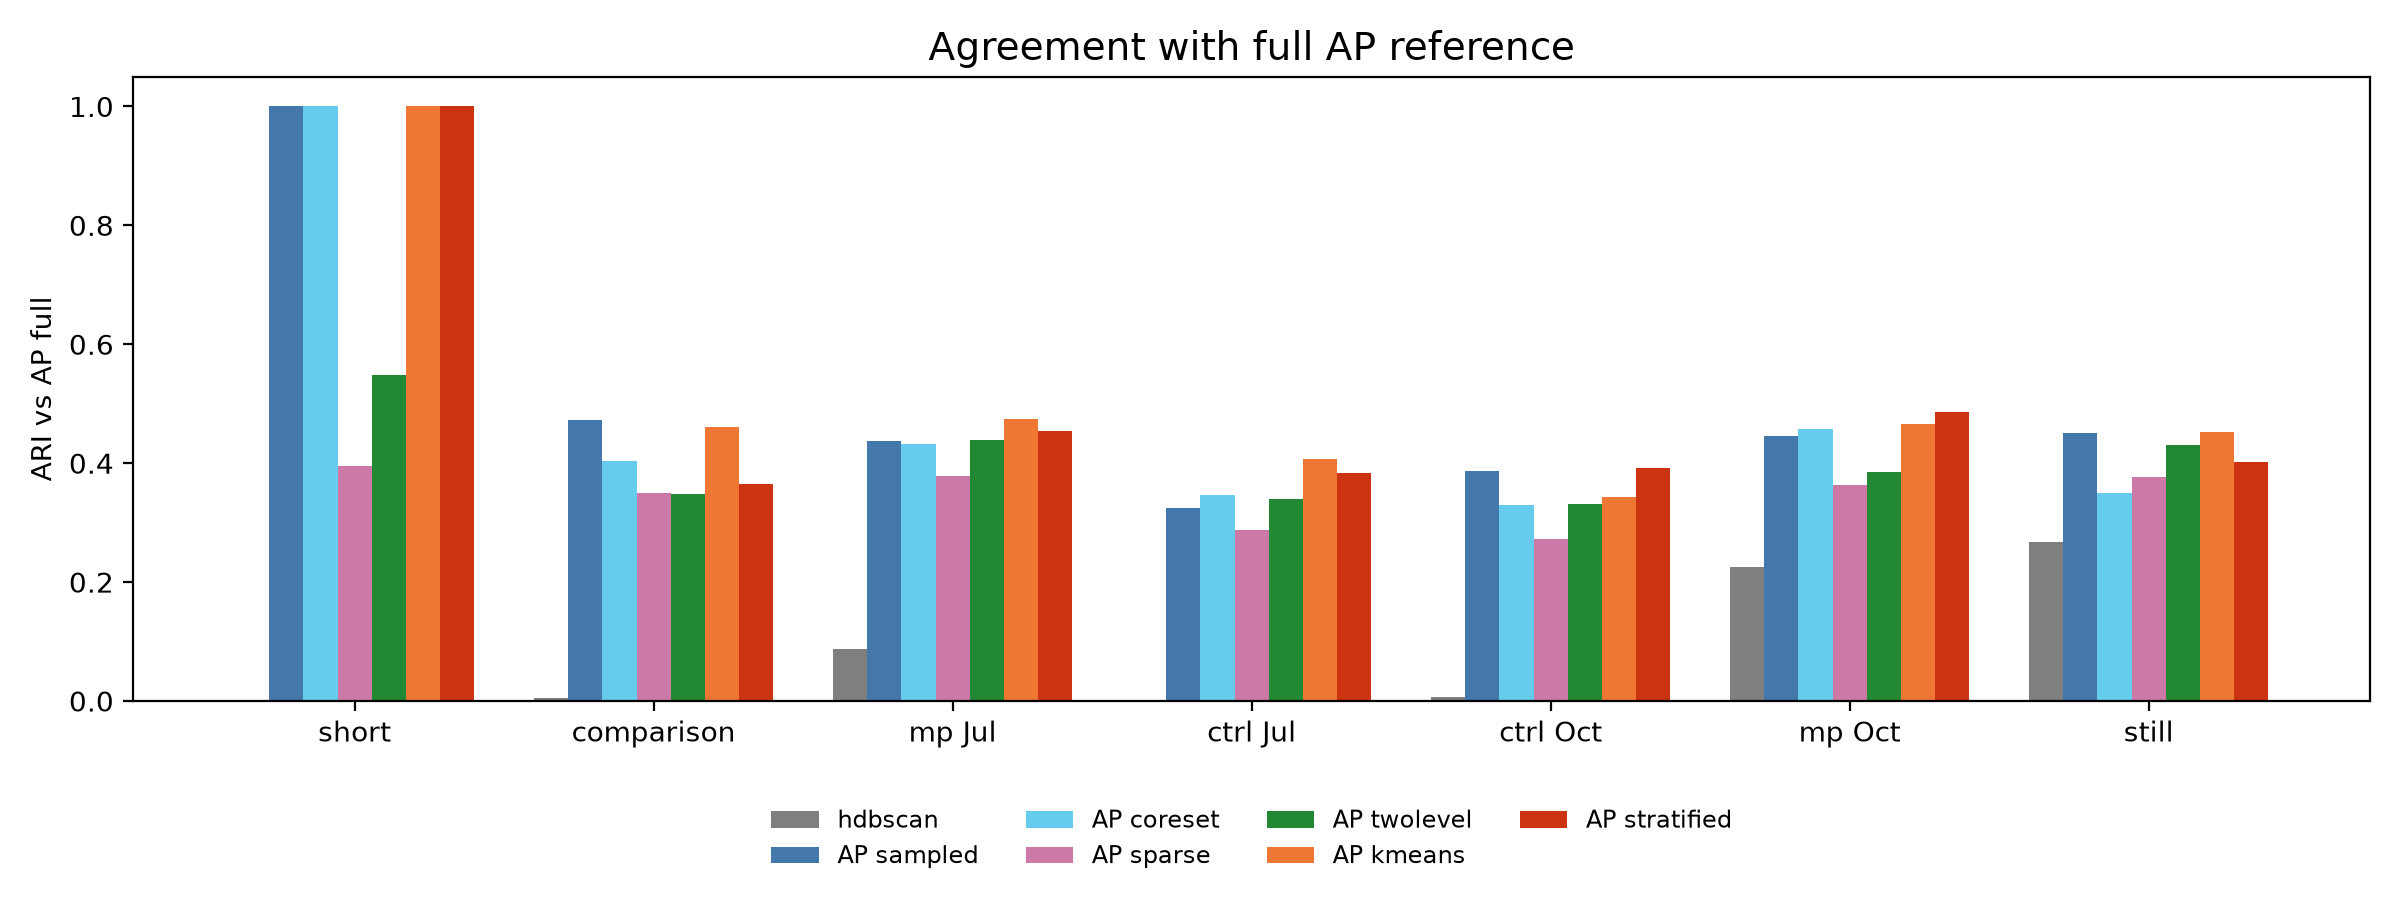
\includegraphics[width=0.95\textwidth]{figures/ari_vs_ap_full.png}
\caption{Agreement with full AP measured by ARI. HDBSCAN has low agreement with full AP because it optimizes a density-based objective rather than an exemplar-based AP objective.}
\label{fig:ari-vs-ap}
\end{figure}

\subsection{Runtime}

Table~\ref{tab:timing} reports wall-clock runtime on a single CPU core, measured directly for every method on every dataset in one version-pinned batch run (no timings are estimated or extrapolated). AP Full is the slowest method by a wide margin -- 150--220\,s on the six datasets between 13,799 and 23,906 windows -- and is not run at all above the 25,000-window threshold. Among scalable methods, HDBSCAN is fastest, followed by AP Two-level and AP Coreset; AP Sampled, AP K-Means, and AP Stratified are moderate (15--50\,s); AP Sparse is consistently the slowest scalable method, exceeding AP Full's own runtime on \texttt{mp\_mouse\_1\_oct} (169\,s) due to its large approximate KNN graph construction step.

\begin{table}[h]
\centering
\caption{Wall-clock runtime per dataset and method on a single CPU core. A dash indicates AP Full was skipped ($N > 25{,}000$).}
\label{tab:timing}
\scriptsize
\setlength{\tabcolsep}{4pt}
\begin{tabular}{lrcccccccc}
\toprule
Dataset & $N$ & \rotatebox{90}{\,HDBSCAN\,} & \rotatebox{90}{\,AP Full\,} & \rotatebox{90}{\,AP Sampled\,} & \rotatebox{90}{\,AP Coreset\,} & \rotatebox{90}{\,AP Two-level\,} & \rotatebox{90}{\,AP Sparse\,} & \rotatebox{90}{\,AP K-Means\,} & \rotatebox{90}{\,AP Stratified\,} \\
\midrule
\texttt{short\_comparison\_test} & 1,195 & $<$0.1\,s & 0.2\,s & 0.2\,s & 0.2\,s & 0.1\,s & 0.3\,s & 0.2\,s & 0.2\,s \\
\texttt{comparison\_test} & 13,799 & 1.9\,s & 55.1\,s & 17.8\,s & 22.6\,s & 16.1\,s & 14.6\,s & 32.1\,s & 27.5\,s \\
\texttt{mp\_mouse\_1\_jul} & 19,714 & 2.4\,s & 150.9\,s & 34.5\,s & 27.2\,s & 23.6\,s & 53.7\,s & 47.6\,s & 35.2\,s \\
\texttt{control\_mouse\_1\_jul} & 23,902 & 3.4\,s & 196.3\,s & 21.5\,s & 24.4\,s & 26.4\,s & 73.0\,s & 34.3\,s & 23.2\,s \\
\texttt{control\_mouse\_1\_oct} & 23,906 & 3.3\,s & 218.8\,s & 24.4\,s & 22.8\,s & 32.4\,s & 99.1\,s & 32.2\,s & 16.3\,s \\
\texttt{mp\_mouse\_1\_oct} & 23,866 & 2.4\,s & 214.2\,s & 51.6\,s & 23.5\,s & 25.7\,s & 168.6\,s & 48.8\,s & 26.3\,s \\
\texttt{still\_test} & 23,877 & 2.2\,s & 177.2\,s & 19.5\,s & 26.3\,s & 24.2\,s & 46.4\,s & 48.6\,s & 21.0\,s \\
\texttt{moving\_test} & 47,028 & 5.7\,s & -- & 46.9\,s & 31.7\,s & 65.3\,s & 153.7\,s & 31.3\,s & 33.8\,s \\
\bottomrule
\end{tabular}
\end{table}

\subsection{Downstream Behavioral Agreement}
\label{sec:downstream-agreement}

ARI alone measures whether two labelings group the same windows together; it does not guarantee that behavioral summaries computed from those labels agree. Because AP full and AP sampled are independent runs, their cluster IDs are not directly comparable, so clusters are first matched via Hungarian assignment on their window-overlap contingency table (maximizing total overlap) before any of the metrics below are computed. For the seven datasets with a full-AP reference, Table~\ref{tab:downstream} reports four such metrics between AP sampled and AP full: the Pearson correlation of per-cluster occupancy (fraction of time in each behavior) and of the flattened first-order transition matrix, both with bootstrap 95\% confidence intervals (1,000 resamples over matched cluster pairs); frame-level raster agreement (the fraction of windows where AP sampled's label, translated through the cluster matching, equals AP full's label at that same window); and the fraction of AP-full exemplars whose nearest AP-sampled exemplar is the identical window.

\begin{figure}[h]
\centering
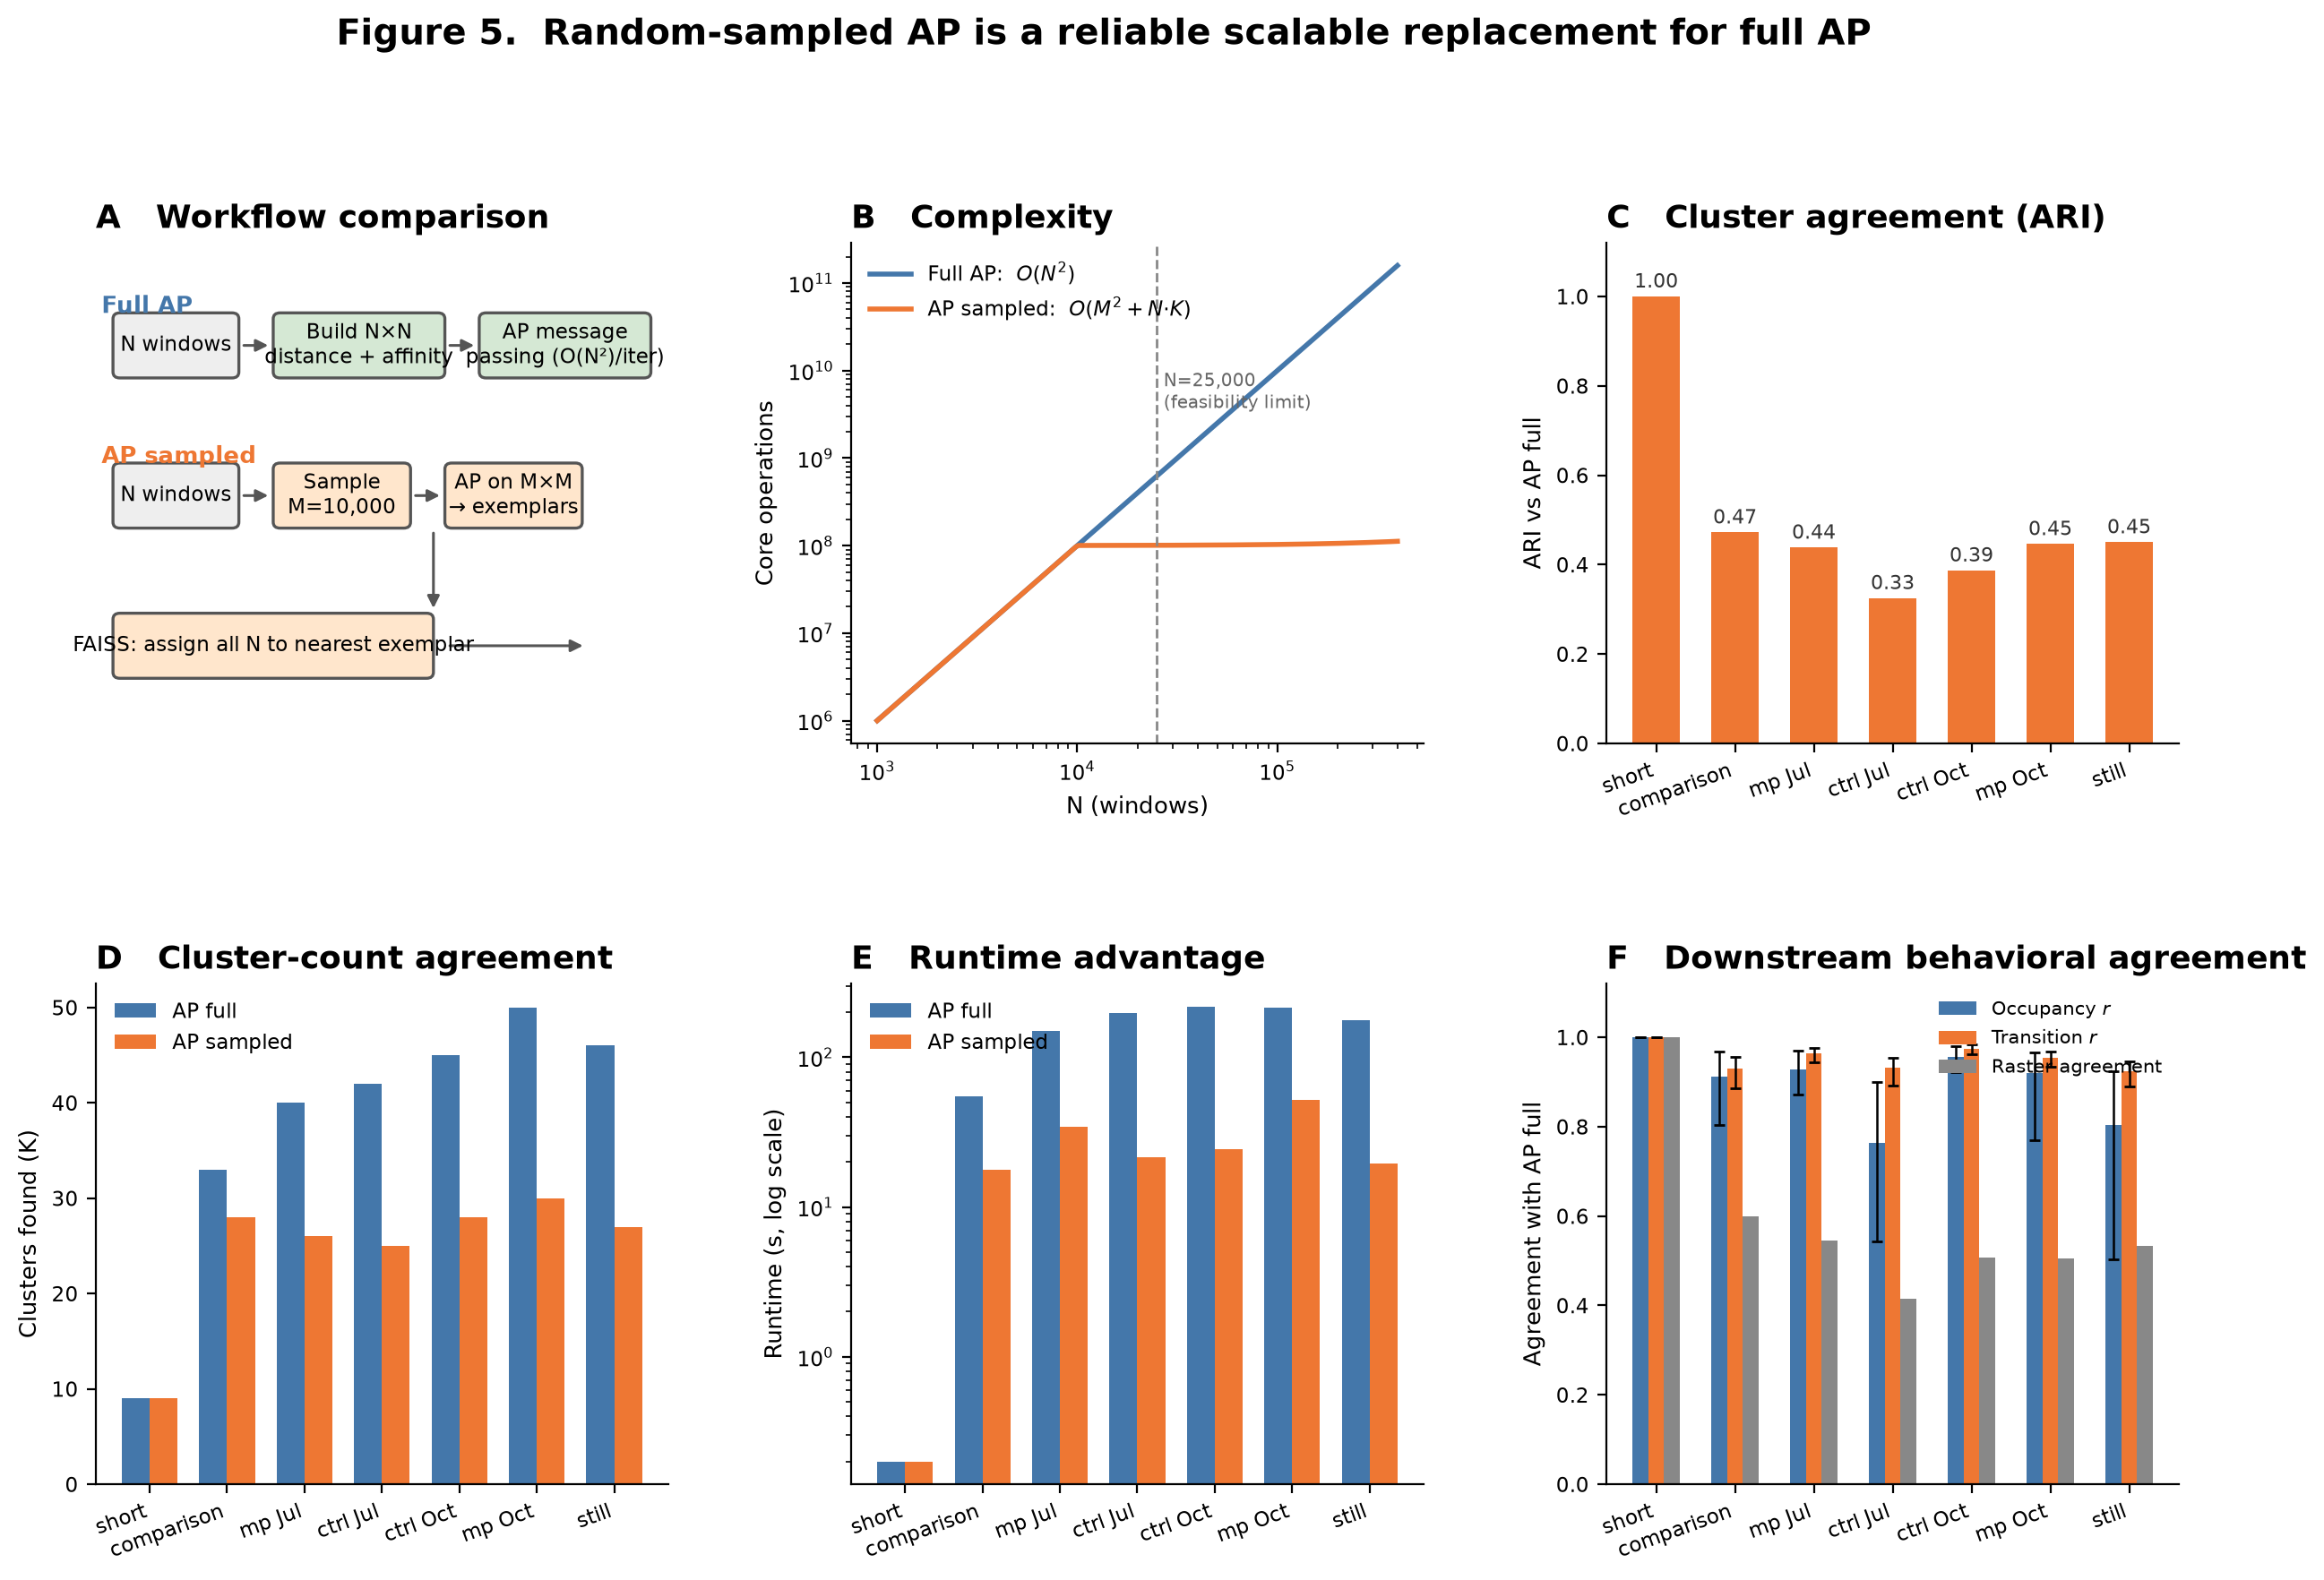
\includegraphics[width=\textwidth]{figures/fig5_downstream.png}
\caption{Random-sampled AP as a scalable replacement for full AP, summarized across the results of Sections~\ref{sec:results}--\ref{sec:downstream-agreement}. (A) Workflow: full AP builds a dense $N \times N$ affinity matrix and runs message passing over all $N$ windows; AP sampled runs the same message passing on a fixed-size sample of $M = 10{,}000$ windows and assigns every window to its nearest exemplar via FAISS. (B) The resulting complexity gap: full AP is $O(N^2)$; AP sampled is $O(M^2 + N \cdot K)$, effectively flat past $N \approx 10{,}000$. (C) ARI between AP sampled and AP full (Table~\ref{tab:ari}). (D) Cluster counts found by each method (Tables~\ref{tab:cluster-counts}, \ref{tab:ari}). (E) Wall-clock runtime, log scale (Table~\ref{tab:timing}). (F) Downstream behavioral agreement (Table~\ref{tab:downstream}): occupancy and transition-matrix correlation (error bars are the 95\% bootstrap CI) stay near 0.9--1.0, while frame-level raster agreement is substantially lower, showing that AP sampled preserves population-level statistics without reproducing full AP's frame-by-frame labeling.}
\label{fig:downstream-summary}
\end{figure}

\begin{table}[h]
\centering
\caption{Downstream agreement between AP sampled and AP full. $K$ full/sampled/matched are the cluster counts from each method and the number of matched pairs found by Hungarian assignment. Occupancy and transition columns show the point estimate with the 95\% bootstrap CI in brackets.}
\label{tab:downstream}
\scriptsize
\setlength{\tabcolsep}{4pt}
\begin{tabular}{lccccc}
\toprule
Dataset & $K$ (full/sampled/matched) & Occupancy $r$ & Transition $r$ & Raster agree. & Exemplar match \\
\midrule
\texttt{short\_comparison\_test} & 9 / 9 / 9 & 1.000 [1.00, 1.00] & 1.000 [1.00, 1.00] & 100.0\% & 100.0\% \\
\texttt{comparison\_test} & 33 / 28 / 28 & 0.911 [0.80, 0.97] & 0.930 [0.89, 0.96] & 59.9\% & 33.3\% \\
\texttt{control\_mouse\_1\_jul} & 42 / 25 / 25 & 0.764 [0.54, 0.90] & 0.931 [0.89, 0.95] & 41.5\% & 9.5\% \\
\texttt{control\_mouse\_1\_oct} & 45 / 28 / 28 & 0.956 [0.92, 0.98] & 0.975 [0.96, 0.98] & 50.8\% & 8.9\% \\
\texttt{mp\_mouse\_1\_jul} & 40 / 26 / 26 & 0.927 [0.87, 0.97] & 0.965 [0.94, 0.98] & 54.6\% & 10.0\% \\
\texttt{mp\_mouse\_1\_oct} & 50 / 30 / 30 & 0.919 [0.77, 0.97] & 0.955 [0.93, 0.97] & 50.5\% & 2.0\% \\
\texttt{still\_test} & 46 / 27 / 27 & 0.803 [0.50, 0.92] & 0.923 [0.89, 0.95] & 53.4\% & 2.2\% \\
\bottomrule
\end{tabular}
\end{table}

Occupancy and transition-matrix correlation both sit around 0.9--1.0 on every dataset except the trivially small \texttt{short\_comparison\_test} case: AP sampled reproduces AP full's \emph{population-level} behavioral statistics almost exactly, which is the evidence that most directly supports using AP sampled as the default scalable method. Frame-level raster agreement and exemplar identity tell a different story -- raster agreement sits near 50\% and exemplar identity is as low as 2--10\% on most datasets -- meaning the two methods frequently assign \emph{individual windows} to different specific clusters, or select different representative windows as exemplars, even while the aggregate statistics that matter for behavioral comparison converge. AP sampled should therefore be trusted for population-level summaries (occupancy, transition structure) but not for frame-level or single-instance cluster identity.

\textit{Caveat on this table:} three of the seven datasets here (\texttt{control\_mouse\_1\_jul/oct}, \texttt{mp\_mouse\_1\_oct}) are drawn from the MitoPark disease-progression cohort. If this analysis is folded into a manuscript that also makes disease-progression claims, replacing these with open-field-only recordings avoids diluting the biological novelty of a future MitoPark-focused paper.

\subsection{Main Observations}

Random-sampled AP remains the most reliable general-purpose replacement for full AP: it runs in under a minute on every tested dataset (17--52\,s across the six non-trivial datasets) and achieves ARI between 0.325 and 0.472 on the seven datasets where full AP is now available (up from three datasets in the previous version of this report; Section~\ref{sec:downstream-agreement} additionally shows it reproduces full AP's occupancy and transition-matrix statistics with $r \approx 0.9$--$1.0$). No single sampled variant dominates every dataset, though: k-means and stratified sampling each exceed random sampling's ARI on several datasets---stratified reaches 0.486 versus 0.446 for random on \texttt{mp\_mouse\_1\_oct}, and k-means reaches 0.407 versus 0.325 for random on \texttt{control\_mouse\_1\_jul}---so they are worth considering when sample composition matters.

Coreset sampling shows a different trade-off: it tends to improve silhouette (notably on \texttt{mp\_mouse\_1\_jul} and \texttt{moving\_test}) but does not always improve ARI. The greedy farthest-point selection covers the feature space more uniformly, which helps geometric separation but does not necessarily match the exemplars that full AP would choose.

Sparse AP consistently over-fragments. With full AP now computed on seven datasets, the cluster-count ratio is consistently 2--3$\times$ higher than full AP (from 2.1$\times$ on \texttt{short\_comparison\_test} to 3.2$\times$ on the two \texttt{control\_mouse\_1} sessions), and this is not easily fixed by tuning---it is a consequence of the graph structure (Section~\ref{sec:clustering-methods}). It is also the slowest scalable method on five of the eight datasets. It is retained for completeness but is not recommended for production use.

HDBSCAN occasionally achieves higher silhouette than any AP variant (e.g.\ \texttt{moving\_test}: 0.574), but its ARI against full AP is essentially zero on most datasets (including exactly 0.000 on \texttt{control\_mouse\_1\_jul}), and it assigns 54--66\% of windows as noise on high-activity datasets. It reflects a genuinely different objective and should be treated as a separate exploratory tool rather than a drop-in replacement.

\FloatBarrier
\section{Discussion}

\subsection{Recommended Current Method}

Random-sampled AP is the current recommended default for replacing the MATLAB pipeline. It runs in 17--52\,s on all tested datasets, stays close to full AP where comparison is possible, and reproduces full AP's population-level occupancy and transition statistics with $r \approx 0.9$--$1.0$ (Section~\ref{sec:downstream-agreement}). For applications where rare behavioral motifs---tremor, impaired gait---are scientifically important, stratified or coreset sampling is preferable: both ensure that small behavioral clusters are represented in the AP sample regardless of how infrequently they occur. K-means sampling is a reasonable middle ground that selects cluster-central rather than boundary points and showed the best ARI on \texttt{mp\_mouse\_1\_jul} and \texttt{control\_mouse\_1\_jul}.

Full AP remains the ground-truth reference and should be run whenever $N$ is small enough (under $\sim$25,000 windows on a machine with 18+ GB RAM; this threshold was raised from 20,000/12\,GB after moving to a 48\,GB machine, and is set conservatively below the point where full AP's four simultaneous $N \times N$ matrices would exceed available memory).

\subsection{Limitations}
\label{sec:limitations}

The histogram representation throws away temporal structure within each 300\,ms window. Two windows with the same amplitude distribution but different within-window dynamics look identical to the pipeline---this is likely fine for coarse locomotor categories but could miss rhythmic features like tremor. The fixed MATLAB-derived bin edges are another constraint: they were calibrated for specific arena and sensor configurations, and may not be optimal for MitoPark mice where disease alters the distribution of accelerations.

A less obvious limitation is that silhouette score rewards geometric compactness, which is not the same as biological meaningfulness. HDBSCAN's high silhouette on some datasets reflects the fact that it discards ambiguous windows as noise, not that its clusters are more biologically valid. Downstream validation---e.g.\ comparing cluster usage between control and MitoPark mice across weeks---is the real test that silhouette cannot replace; Section~\ref{sec:downstream-agreement} is a first step in that direction, though it validates AP sampled against AP full rather than against ground-truth behavioral labels.

A reproducibility limitation surfaced directly while preparing this version of the report: re-running AP full on \texttt{mp\_mouse\_1\_jul} in a freshly installed environment (rather than the environment that originally produced the cached results) changed the cluster count from 41 to 40, even though AP full has no randomness beyond a fixed \texttt{random\_state}. This is almost certainly scikit-learn version drift, since the previous \texttt{requirements.txt} did not pin exact package versions. All results in this version of the report come from a single run in an environment with pinned versions (numpy 2.5.2, scipy 1.18.1, pandas 3.0.5, scikit-learn 1.9.0, hdbscan 0.8.44, faiss-cpu 1.15.0), and \texttt{requirements.txt} now records these versions so future re-runs are exactly reproducible. A related issue was found and fixed in \texttt{batch\_compare.py}: AP sampled's preference is only aligned to AP full's exact preference when AP full is freshly computed in the same batch-compare session, so cached or skipped AP-full runs silently left AP sampled using an unaligned, independently estimated preference; this affected the AP-sampled results for four datasets (up to 97\% of window labels differed once corrected) and has been fixed by re-running AP full and AP sampled together for every dataset reported here.

\FloatBarrier
\section{Conclusion}

The pipeline matches the MATLAB AP output on small datasets ($N \leq 25{,}000$, raised from 20,000 in the previous version of this report) and extends cleanly to larger recordings through subsampling. Of the scalable variants, random-sampled AP is the most battle-tested and is now validated not only by ARI but by direct agreement on occupancy and transition statistics (Section~\ref{sec:downstream-agreement}); k-means and stratified sampling remain competitive alternatives, now with full timing data recorded across all eight datasets. The next priorities are: (1) re-verifying MATLAB-vs-Python equivalence under the newly pinned dependency versions, since the environment used to originally generate the MATLAB comparison predates the reproducibility fixes described in Section~\ref{sec:limitations}; (2) resolving whether the MitoPark-derived datasets used in Section~\ref{sec:downstream-agreement} should be replaced with open-field-only recordings if this analysis is folded into a manuscript that also makes disease-progression claims; and (3) an end-to-end run on a long-duration ($\geq$20 hour) recording to demonstrate scalability beyond the current largest dataset (\texttt{moving\_test}, 47,028 windows).

\section*{Implementation Notes}

This document is based on the current local contents of:

\begin{itemize}
    \item \texttt{Python\_Pipeline/scripts/prepare\_test\_data.py}
    \item \texttt{Python\_Pipeline/scripts/clustering\_pipeline.py}
    \item \texttt{Python\_Pipeline/scripts/batch\_compare.py}
    \item \texttt{Python\_Pipeline/scripts/compare\_results.py}
    \item \texttt{Python\_Pipeline/scripts/recompute\_ap\_exemplars.py} -- recovers AP exemplar indices (discarded by \texttt{batch\_compare.py}) and produces a self-consistent (AP full, AP sampled) pair per dataset for Section~\ref{sec:downstream-agreement}
    \item \texttt{Python\_Pipeline/scripts/fig5f\_downstream\_agreement.py} -- computes the cluster matching, occupancy/transition correlation, raster agreement, and exemplar-overlap metrics in Table~\ref{tab:downstream}
    \item \texttt{Python\_Pipeline/requirements.txt} -- now pins exact package versions (see Section~\ref{sec:limitations})
    \item \texttt{Python\_Pipeline/results/method\_comparison.csv}
    \item \texttt{Python\_Pipeline/results/method\_comparison\_report.txt}
    \item \texttt{Python\_Pipeline/results/fig5f\_downstream\_agreement.csv}
\end{itemize}

\begin{thebibliography}{9}

\bibitem{frey2007}
Frey, B.~J. and Dueck, D. (2007).
Clustering by passing messages between data points.
\textit{Science}, 315(5814):972--976.

\bibitem{johnson2021}
Johnson, J., Douze, M., and J\'{e}gou, H. (2021).
Billion-scale similarity search with {GPU}s.
\textit{IEEE Transactions on Big Data}, 7(3):535--547.

\bibitem{campello2013}
Campello, R.~J.~G.~B., Moulavi, D., and Sander, J. (2013).
Density-based clustering based on hierarchical density estimates.
In \textit{Pacific-Asia Conference on Knowledge Discovery and Data Mining}, pages 160--172.

\bibitem{rubner2000}
Rubner, Y., Tomasi, C., and Guibas, L.~J. (2000).
The earth mover's distance as a metric for image retrieval.
\textit{International Journal of Computer Vision}, 40(2):99--121.

\bibitem{rousseeuw1987}
Rousseeuw, P.~J. (1987).
Silhouettes: A graphical aid to the interpretation and validation of cluster analysis.
\textit{Journal of Computational and Applied Mathematics}, 20:53--65.

\bibitem{hubert1985}
Hubert, L. and Arabie, P. (1985).
Comparing partitions.
\textit{Journal of Classification}, 2(1):193--218.

\bibitem{pedregosa2011}
Pedregosa, F. et al. (2011).
Scikit-learn: Machine learning in {Python}.
\textit{Journal of Machine Learning Research}, 12:2825--2830.

\end{thebibliography}

\end{document}
